% !TEX encoding = UTF-8
% !TEX TS-program = pdflatex
% !TEX root = ../tesi.tex

%**************************************************************
\chapter{Prodotto dello stage}
\label{cap:prodotto-stage}
%**************************************************************

\intro{
    In questo capitolo viene presentato il processo decisionale che ha portato alla scelta dell'architettura software alla base del prodotto realizzato e quali erano state considerate per svolgere lo stesso scopo. Viene quindi presentata l'organizzazione del \gls{codebaseg} e la sua suddivisione in package, spiegando di ciascuno di questi il significato. Si entra poi in dettaglio di come il pattern Observer è stato fondamentale per lo sviluppo di un'architettura ben organizzata e con compiti precisi. Infine, viene fatto un confronto fra l'applicazione in uso presso l'azienda e quella sviluppata per lo stage, riflettendo sulle modifiche apportate.
}

%**************************************************************
\section{Architetture a confronto}
\label{sec:architetture-confronto}

Prima di procedere con la progettazione delle componenti in dettaglio e della vista si sono analizzati più \gls{designpatterng} architetturali per capire quale fosse il più adeguato per lo scopo.\\
La scelta è stata influenzata da fattori come la facilità di implementazione, la facilità di adattamento a \emph{Flutter} e di conseguenza la disponibilità di esempi.\\
Mentre per sviluppare un'applicazione nativa in Android è consigliato usare l'architettura Model View Presenter e in \emph{Qt} quella Model View (una versione modificata di Model View Controller), per Flutter non c'è ancora una \gls{bestpracticeg} diffusa.

%**************************************************************
\subsection{Model View Controller}
\label{subsec:model-view-controller}

Il \emph{Model View Controller (MVC)} è un tipo di architettura molto famosa e molto implementata, ma spesso in maniera errata.\\
Permette di avere, nel proprio sistema, tre componenti che hanno compiti distinti (e lo stesso vale per le altre architetture).\\
In MVC:
\begin{itemize}
    \item il \emph{Model} rappresenta il modello dei dati, ovvero tutto ciò che implementa la \emph{business logic}, comprese le operazioni sui dati (lettura e scrittura da supporti di persistenza e da remoto). Quando viene aggiornato, si occupa di notificare la \emph{View} (tramite il \gls{designpatterng} Observer\footnote{Per maggiori informazioni su Observer, consultare alla sotto-sezione "\hyperref[subsec:observer-provider-changenotifier]{Il design pattern Observer: Provider, ChangeNotifier e Consumer}".});
    \item la \emph{View} rappresenta la parte di \emph{presentation logic}, ovvero ciò che permette di interagire con l'utente. Gli input dell'utente vengono catturati e inoltrati al \emph{Controller};
    \item il \emph{Controller} rappresenta la parte di \emph{application logic} poiché seleziona la \emph{View} corretta in base all'input e inoltra i dati dell'interazione dell'utente al \emph{Model}.
\end{itemize}
Questa architettura è facilmente applicabile in \emph{Flutter}, poiché la vista è correttamente separata dal modello e si gestisce autonomamente il proprio aggiornamento (ad eccezione della selezione che la fa il \emph{Controller}).\\
Sebbene siano separati, la dipendenza della vista dal modello non li rende completamente separati per cui il modello, dovendo fornire metodi per le richieste provenienti dalla vista, dovrebbe già preparare i dati in un formato adeguato, rendendolo più complesso.

\begin{figure}[!h]
    \centering 
    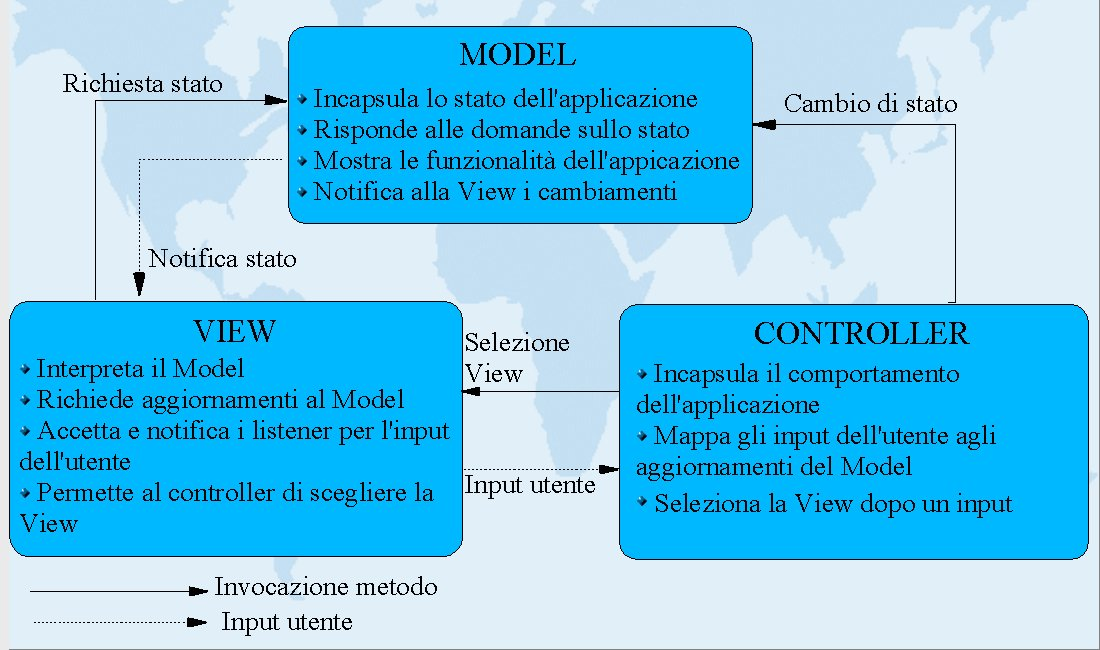
\includegraphics[width=0.9\columnwidth]{capitolo-6/architetture-confrontro/mvc} 
    \caption{Diagramma dell'architettura MVC (da \cite{site:mvc})}
\end{figure}

%**************************************************************
\subsection{Model View Presenter}
\label{subsec:model-view-presenter}

Il \emph{Model View Presenter (MVP)} è invece un'architettura in cui il modello e la vista sono due entità completamente separate e fra di loro sconosciute.\\
Più in dettaglio:
\begin{itemize}
    \item il \emph{Model} rappresenta il modello dei dati, ovvero tutto ciò che implementa la \emph{business logic}, comprese le operazioni sui dati (lettura e scrittura da supporti di persistenza e da remoto). Non notifica la \emph{View} in caso di aggiornamento, ma chiama il \emph{Presenter};
    \item la \emph{View} rappresenta la pura interfaccia di visualizzazione per l'utente (è passiva) oppure può anche contattare il \emph{Presenter} in caso di eventi, in base all'implementazione;
    \item il \emph{Presenter} agisce da "Man in the middle" poiché fa da passacarte fra la \emph{View} e il \emph{Model}. A meno che non sia la \emph{View} stessa a chiamarlo, resta in ascolto di notifiche da parte di entrambi e aggiorna lo stato dell'applicazione o della vista in base alle necessità.
\end{itemize}
Con questo approccio c'è una separazione dei compiti importante ma è richiesto che il \emph{Presenter} si occupi dell'aggiornamento della vista, rendendolo poco adatto a \emph{Flutter}.

\begin{figure}[!h]
    \centering 
    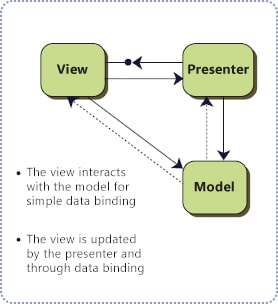
\includegraphics[width=0.5\columnwidth]{capitolo-6/architetture-confrontro/mvp} 
    \caption{Diagramma dell'architettura MVP (da \cite{site:mvp})}
\end{figure}

%**************************************************************
\subsection{Model View ViewModel}
\label{subsec:model-view-viewmodel}

Il \emph{Model View ViewModel (MVVM)} è un'architettura che consente di separare il modello e la vista utilizzando un doppio Observer.\\
Più specificatamente:
\begin{itemize}
    \item il \emph{Model} è il medesimo dell'architettura MVP;
    \item la \emph{View} è la medesima dell'architettura MVC, ma chiaramente in caso di input viene contattato un \emph{ViewModel} e non un \emph{Controller};
    \item il \emph{ViewModel} è il "modello della vista", ovvero il \emph{Model} accinge solo da questo, che accinge a sua volta solo dal \emph{Model}.
\end{itemize}
In MVVM, la \emph{View} è spesso implementata dichiarativamente (e questo è un punto a favore per \emph{Flutter}).\\
Come è stato detto, la \emph{View} può sfruttare il proprio \emph{ViewModel} per ottenere i dati da visualizzare e il \emph{ViewModel} a sua volta utilizza il proprio \emph{Model}.
Essendo implementato il \gls{designpatterng} Observer, quando il \emph{Model} e il \emph{ViewModel} hanno nuovi dati notificano i propri listener (che sono rispettivamente delle \emph{View} e dei \emph{ViewModel}), senza sapere chi è il destinatario.\\

\begin{figure}[!h]
    \centering 
    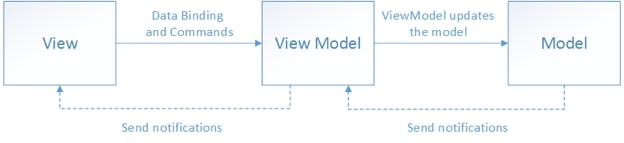
\includegraphics[width=0.7\columnwidth]{capitolo-6/architetture-confrontro/mvvm} 
    \caption{Diagramma dell'architettura MVVM (da \cite{site:mvvm})}
\end{figure}

%**************************************************************
\subsection{Clean Architecture}
\label{subsec:clean-architecture}

La \emph{Clean Architecture} si differenza molto dalle altre tre perché si concentra su una cosa fondamentale: le \textbf{dipendenze} e come \textbf{minimizzarle}.\\
In questo tipo di architettura le dipendenze vanno solo in un verso, che nel diagramma dell'architettura corrisponde dall'esterno all'interno degli strati del cerchio.\\
Più in dettaglio, questa architettura si compone di quattro macro-livelli:
\begin{itemize}
    \item \emph{Entities}, che sono entità gestite da regole di business (per esempio i prodotti gestiti da un'azienda), potenzialmente riusabili in più applicazioni dell'organizzazione, e che hanno meno probabilità di cambiare se cambia il funzionamento del sistema;
    \item \emph{Use cases}, che gestiscono la \emph{business logic} dell'applicazione seguendo i casi d'uso specifici. Ha dipendenze solo verso il livello \emph{Entities} ed è isolato dal resto (modifiche a livelli sovrastanti non ne richiedono la modifica);
    \item \emph{Interface adapters}, che contiene tutti gli adattatori (tra cui i già citati \emph{Controller}, \emph{Presenter}) fra le regole di business (livello \emph{Use cases}) e i dati provenienti da interfacce utente, remoto, file, database (livello \emph{Frameworks and Drivers});
    \item \emph{Frameworks and Drivers} contiene infine tutto il codice che dipende da implementazioni di altro software come appunto database, \gls{api} di librerie o in rete. Questo livello contiene tutti i "\textbf{dettagli}" (implementativi).
\end{itemize}
È un architettura sicuramente molto valida e che può garantire una forte separazione delle responsabilità, fondamentale per avere un \gls{codebaseg} mantenibile e scalabile, ma difficile da padroneggiare per un novizio (richiede come minimo una buona conoscenza delle regole di business, cosa che in uno stage non è presente).

\begin{figure}[!h]
    \centering 
    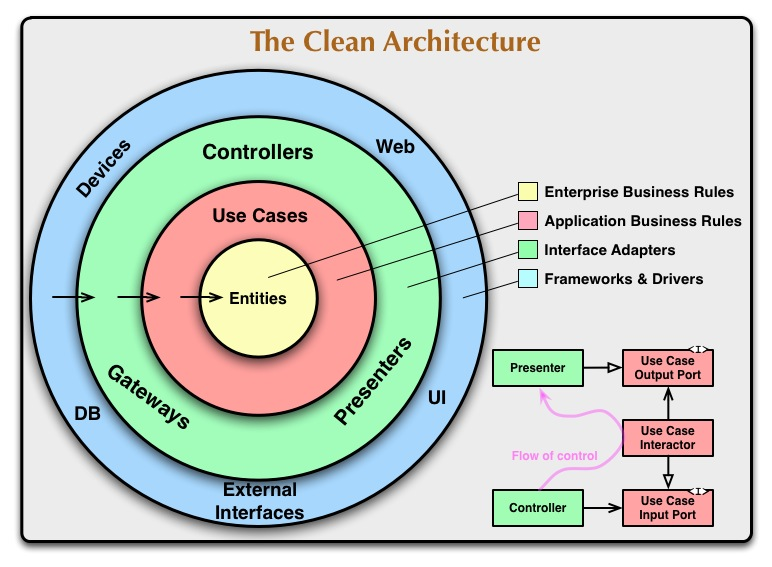
\includegraphics[width=0.8\columnwidth]{capitolo-6/architetture-confrontro/clean-architecture} 
    \caption{Diagramma dell'architettura Clean Architecture (da \cite{site:clean-architecture})}
\end{figure}

%**************************************************************
\section{Model View ViewModel, l'architettura scelta}
\label{sec:architettura-mvvm}

%**************************************************************
\subsection{Ragioni della scelta}
\label{subsec:ragioni-scelta}

Dopo aver analizzato le varie caratteristiche delle architetture presentate nella precedente sezione, è stata scelta l'architettura \emph{Model View ViewModel}.\\
Innanzitutto, \emph{MVVM} è consigliato per alcune delle altre tecnologie multipiattaforma che sono state ipotizzate per realizzare il prodotto di stage, per via della natura dichiarativa con cui viene implementata l'interfaccia utente.
Inoltre, l'utilizzo del \gls{designpatterng} Observer doppiamente permette di garantire un notevole disaccoppiamento fra le tre parti dell'architettura, permettendo di conseguenza una maggior facilità nel testing.\\
Per quanto riguarda le altre architetture, \emph{Model View Presenter} è stata scartata principalmente per la necessità del \emph{Presenter} di aggiornare la vista, che non si trova molto in sintonia con il metodo di rappresentazione dell'interfaccia di \emph{Flutter}.\\
\emph{Model View Controller} non è stato scelto perché il \emph{Model} avrebbe avuto troppi oneri: nel sistema da realizzare per lo stage era necessario memorizzare i dati ottenuti dalle \gls{restg} per poterli utilizzare per più scopi in più viste, quindi richiedendo che in qualche punto dell'architettura ci sia questo tipo di disponibilità (possibilmente non nella \emph{View}).\\
Infine, \emph{Clean Architecture}, come affermato nella sotto-sezione in cui la si illustrava, è certamente una buona architettura ma difficilmente implementabile con l'esperienza avuta fino ad ora. È comunque un'architettura valida e con i dovuti aggiustamenti \emph{MVVM} potrebbe essere adattata a questa.

%**************************************************************
\subsection{Organizzazione dei package}
\label{subsec:organizzazione-package}

%**************************************************************
\subsubsection{Package it.tecsen.smacs}
\label{subsubsec:it-tecsen-smacs}

\begin{figure}[!h] 
  \centering 
  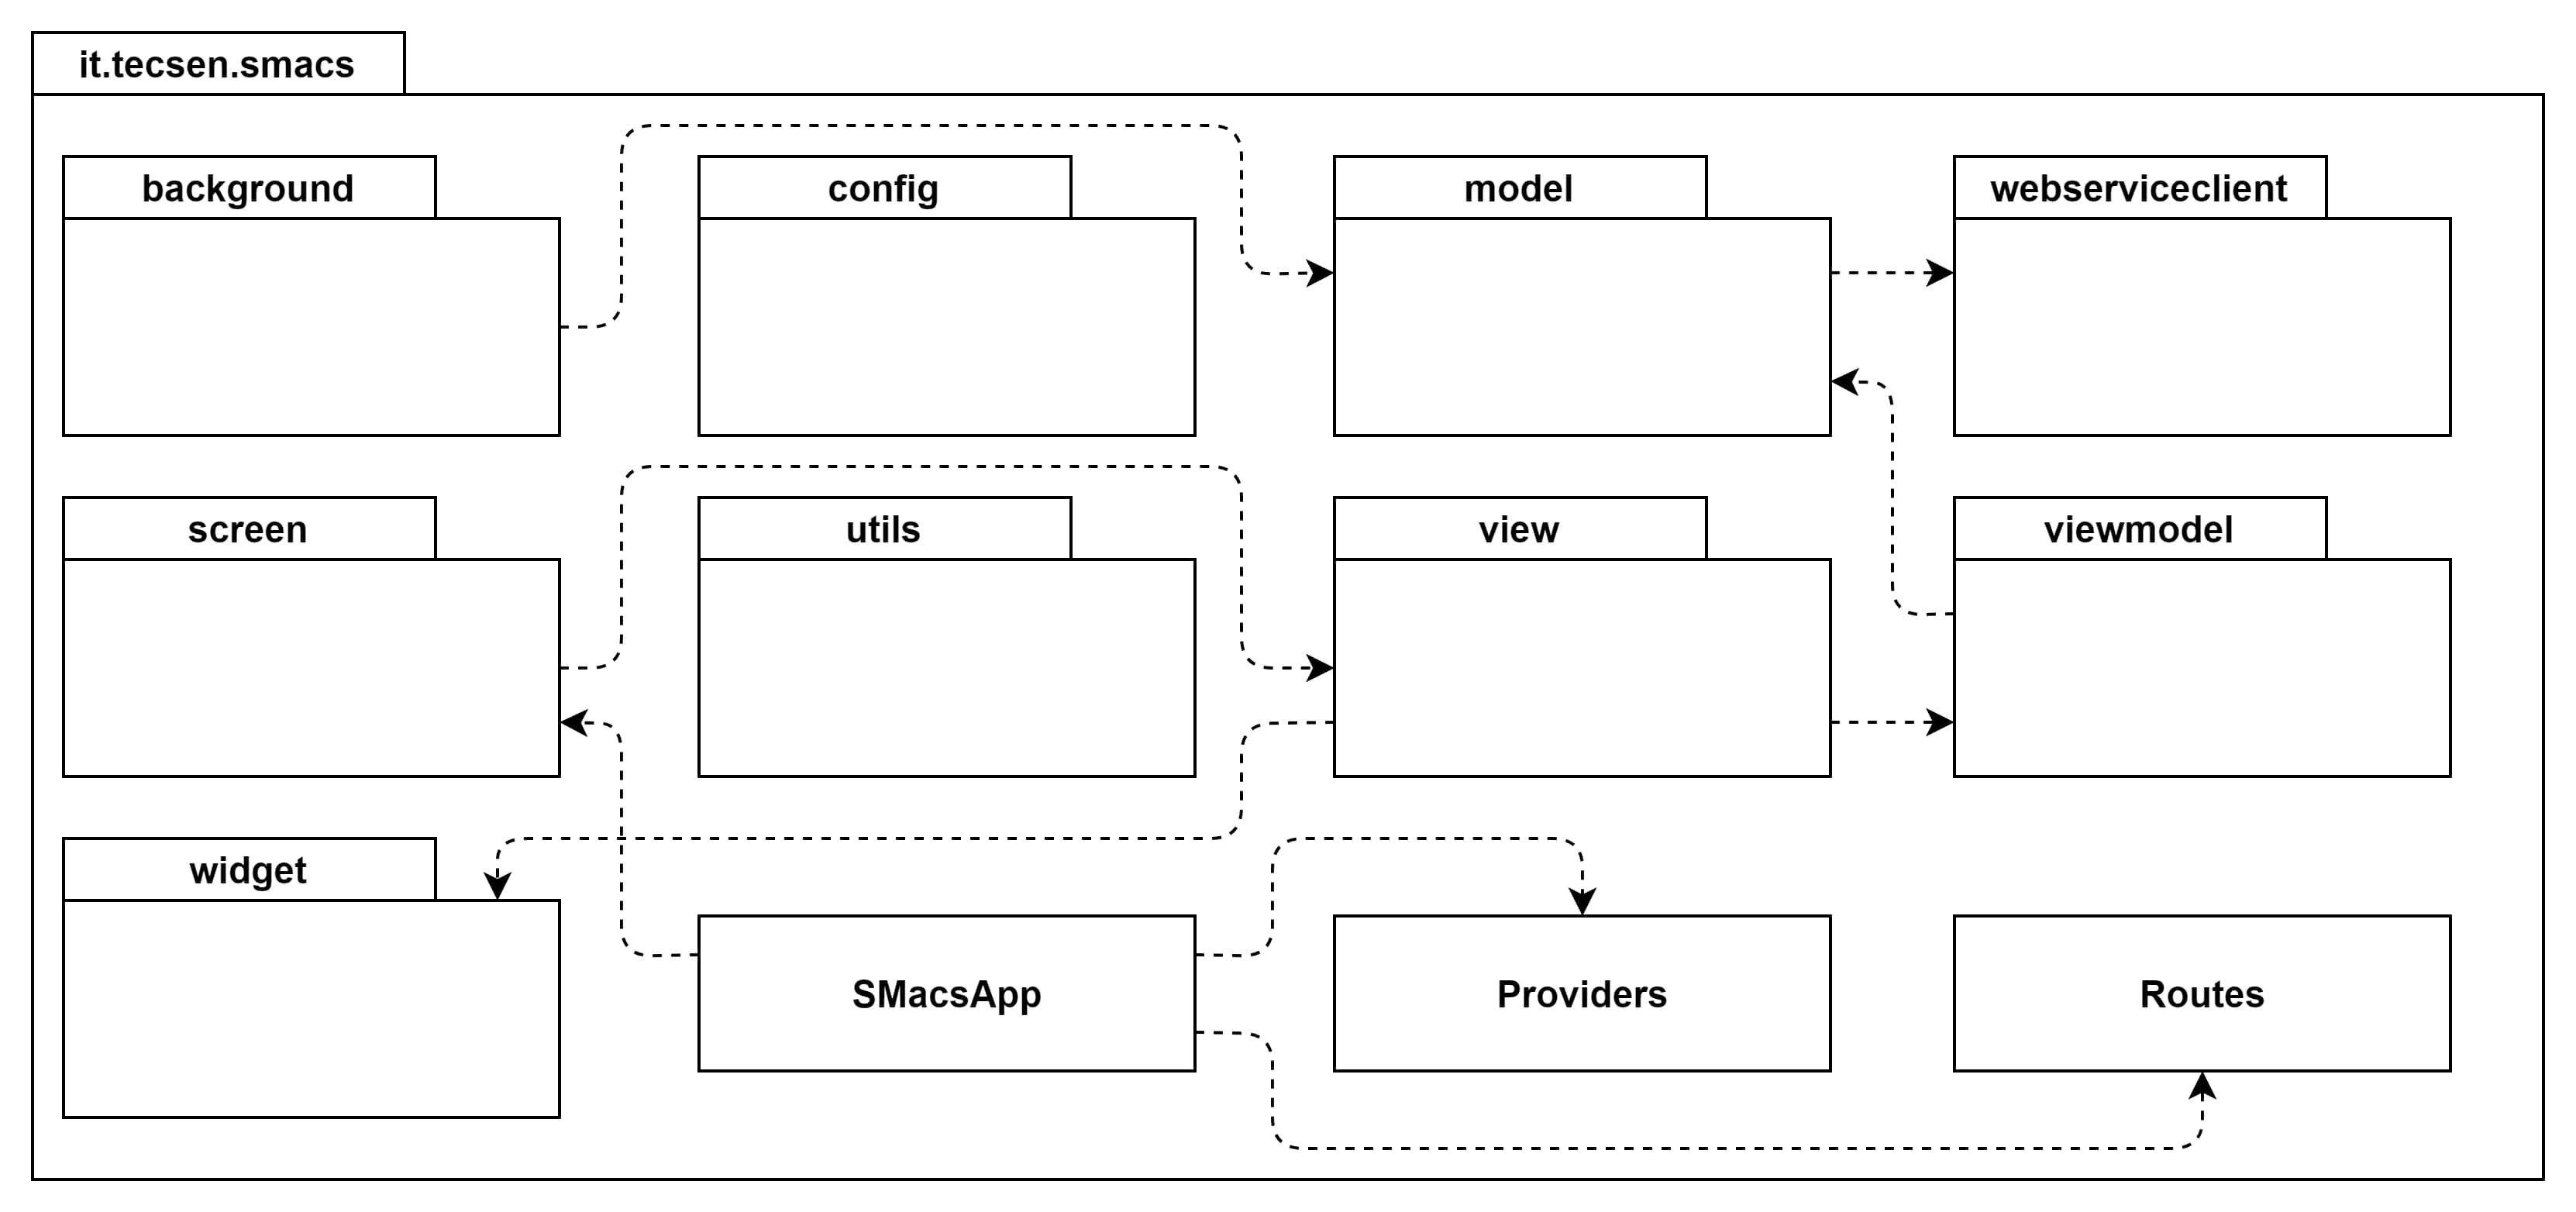
\includegraphics[width=1.0\columnwidth]{capitolo-6/organizzazione-package/it-tecsen-smacs} 
  \caption{Diagramma del package \texttt{it.tecsen.smacs}}
\end{figure}
Il seguente package racchiude tutto il codice sorgente dell'applicazione (non è stato richiesto l'uso del \emph{Platform Channel}), librerie escluse.\\
È suddiviso in più sotto-package seguendo il pattern architetturale Model View ViewModel, per cui sono presenti (come si può vedere nel diagramma sottostante) i package \texttt{model}, \texttt{viewmodel} e \texttt{view}.\\
\textbf{N.B.} Le dipendenze evidenziate nel diagramma sono quelle principali. Ad esempio, quasi tutti i package dipendono da \texttt{utils} e \texttt{config}, dato che contengono rispettivamente classi di utilità e di configurazione, ma non sono state segnate.\\
I package \texttt{screen} e \texttt{widget} fanno sempre parte del concetto \texttt{view} del pattern, ma sono separate dal package \emph{view} per ragioni organizzative:
\begin{itemize}
  \item \texttt{screen} contiene le classi che implementano i widget radice di ogni schermata dell'applicazione. Ognuno di questi widget è ridotto al minimo essenziale per poter poi utilizzare un widget dichiarato nel package \texttt{view} come resto del \emph{Widget tree};
  \item \texttt{widget} contiene le classi che implementano alcuni widget usati dalle classi in \texttt{screen} e \texttt{view}, a scopo di riutilizzo.
\end{itemize}
I package \texttt{model}, \texttt{viewmodel} e \texttt{view} contengono le classi per svolgere il loro ruolo all'interno dell'architettura.\\
Il package \texttt{utils} contiene classi con metodi di utilità (per esempio per il parsing di UUID, per l'hashing di stringhe, per la gestione di date, del logging e altro).\\
Il package \texttt{config} contiene classi con la configurazione dell'app, di alcuni plugin (come quello per la pubblicazione di notifiche), dell'internazionalizzazione e mappe per analizzare i dati ricevuti dalle \gls{restg}.\\
Il package \texttt{webserviceclient} contiene l'implementazione di un semplice wrapper di alcuni metodi della libreria \emph{http}\footcite{site:http-library} per facilitarne l'uso all'interno delle classi del package \texttt{model}.\\
Infine, \texttt{SMacsApp} è la classe che implementa il widget radice dell'intera applicazione e si serve delle classi \texttt{Routes} e \texttt{Providers} in cui sono presenti rispettivamente la configurazione della navigazione all'interno dell'app e le dipendenze di tutte le classi del package \texttt{viewmodel}.


%**************************************************************
\subsubsection{Package it.tecsen.smacs.screen}
\label{subsubsec:it-tecsen-smacs-screen}

% L'immagine dovrebbe essere qui ma per motivi di spazio viene spostata.
In questo package vi sono tutte le classi che implementano i widget radice di ogni schermata dell'applicazione, come è stato precedentemente illustrato in "\hyperref[subsubsec:it-tecsen-smacs]{Package it.tecsen.smacs}".\\
Ogni screen implementa uno o più casi d'uso, disponibili per la consultazione nell'appendice "\hyperref[cap:analisi-dei-requisiti]{Analisi dei requisiti}".
% \\
\clearpage
\begin{figure}[!h]
  \centering 
  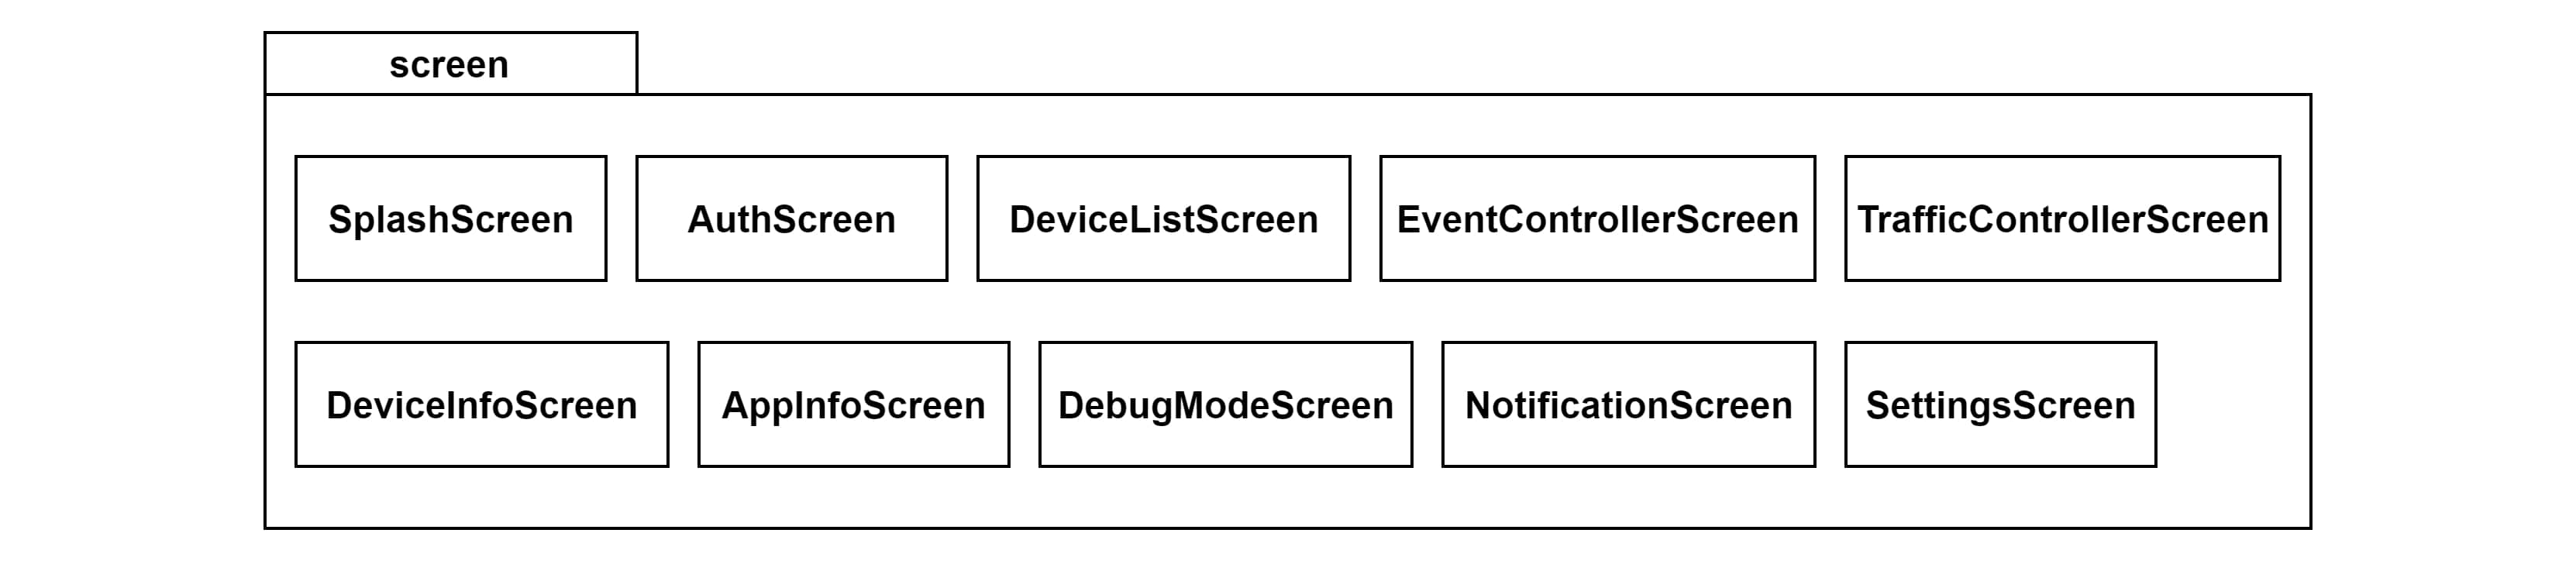
\includegraphics[width=1.0\columnwidth]{capitolo-6/organizzazione-package/screen} 
  \caption{Diagramma del package \texttt{it.tecsen.smacs.screen}}
\end{figure}
In particolare:
{
\renewcommand{\arraystretch}{1.5}
\begin{longtable}{|c|c|}
    \hline
    \textbf{Classe (widget)} & \textbf{Caso (e sotto-casi) d'uso implementati} \\\hline
    \endhead
    SplashScreen & UC01\\\hline
    AuthScreen & UC02 \\\hline
    DeviceListScreen & UC03, UC15 \\\hline
    TrafficControllerScreen & UC04, UC05, UC07, UC09, UC10 \\\hline
    DeviceInfoScreen & UC06 \\\hline
    EventControllerScreen & UC08 \\\hline
    NotificationScreen & UC11 \\\hline
    SettingsScreen & UC12 \\\hline
    AppInfoScreen & UC13 \\\hline
    DebugModeScreen & UC14 \\\hline
    \caption{Correlazione fra classi del package \texttt{screen} e casi d'uso implementati}
\end{longtable}
}


%**************************************************************
\subsubsection{Package it.tecsen.smacs.view}
\label{subsubsec:it-tecsen-smacs-view}

\begin{figure}[!h]
  \centering 
  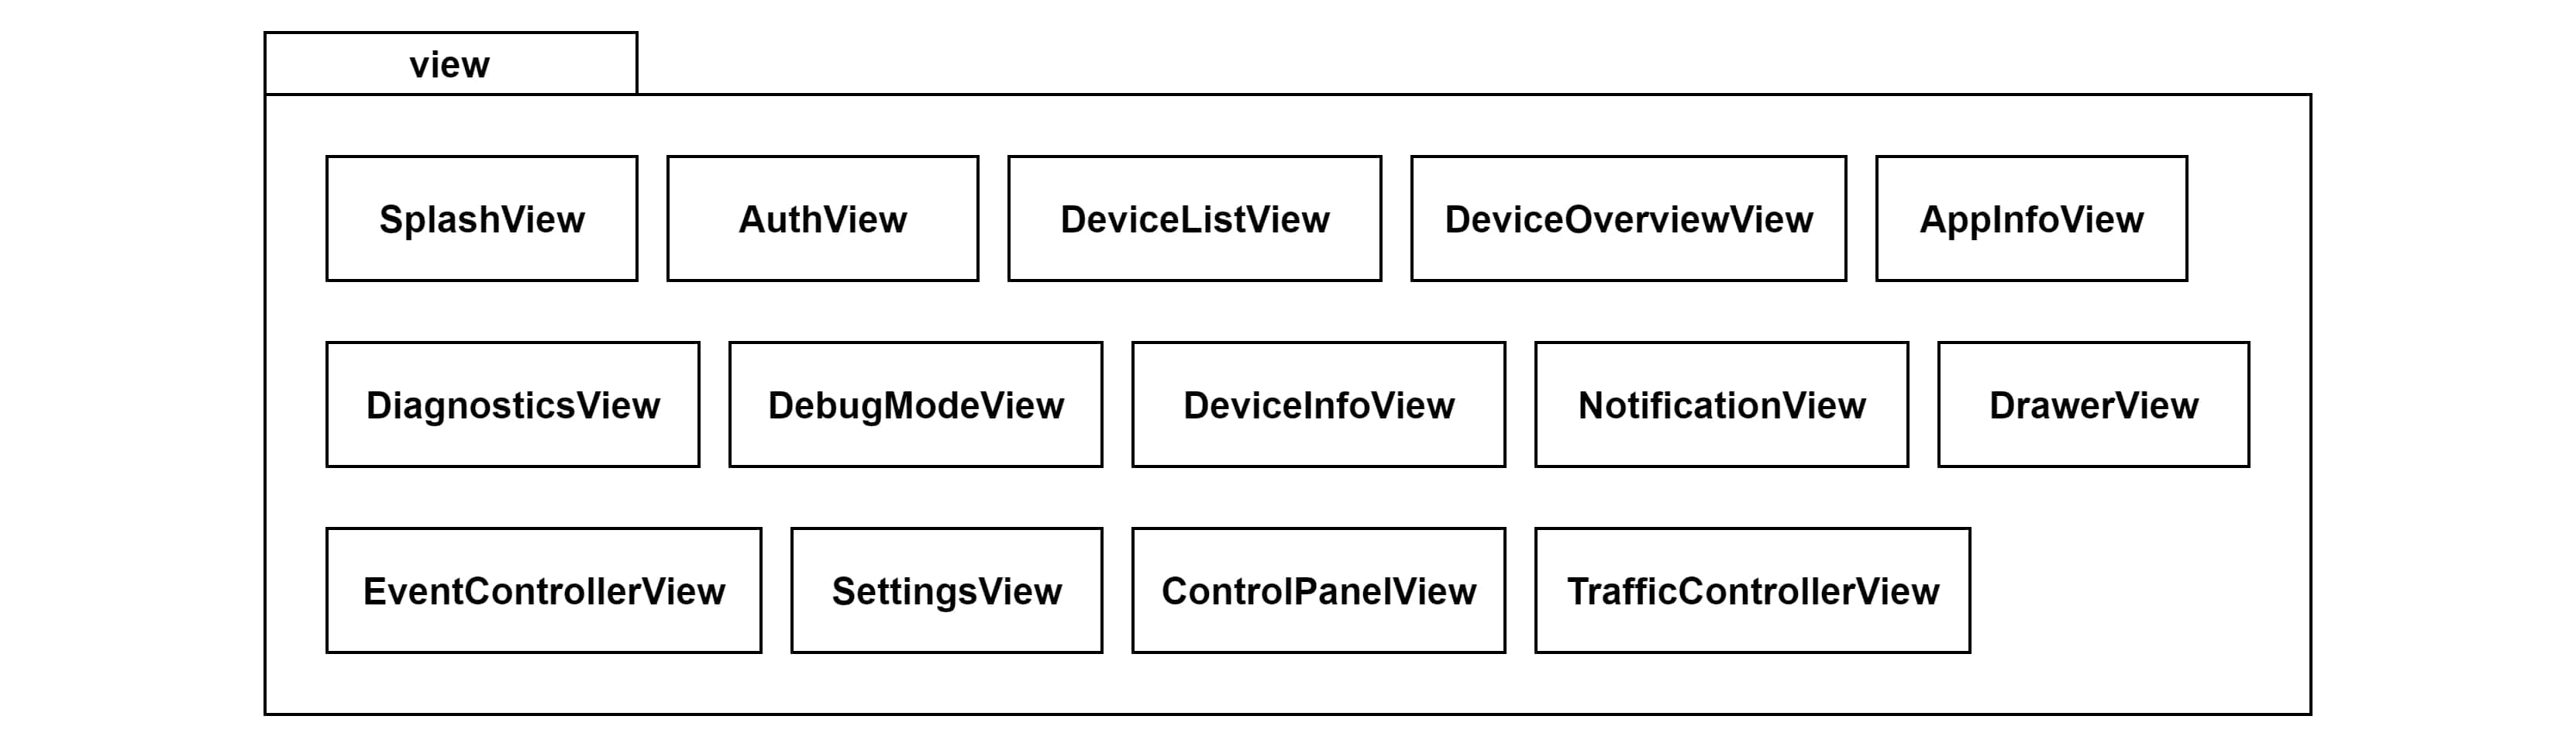
\includegraphics[width=1.0\columnwidth]{capitolo-6/organizzazione-package/view} 
  \caption{Diagramma del package \texttt{it.tecsen.smacs.view}}
\end{figure}
In questo package vi sono tutte le classi che implementano i widget che visualizzano il contenuto per soddisfare i casi d'uso raccolti.\\
Ogni classe implementa uno o più casi d'uso, disponibili per la consultazione nell'appendice "\hyperref[cap:analisi-dei-requisiti]{Analisi dei requisiti}".\\
In particolare:
{
\renewcommand{\arraystretch}{1.5}
\begin{longtable}{|c|c|}
    \hline
    \textbf{Classe (widget)} & \textbf{Caso (e sotto-casi) d'uso implementati} \\\hline
    \endhead
    SplashView & UC01\\\hline
    AuthView & UC02 \\\hline
    DeviceListView & UC03 \\\hline
    DeviceOverviewView & UC04.1, UC04.2, UC04.3, UC04.4, UC04.5, UC05 \\\hline
    DiagnosticsView & UC04.5, UC04.6, UC07.3 \\\hline
    ControlPanelView & UC04.5, UC07.1, UC07.2, UC07.4 \\\hline
    TrafficControllerView & UC04 e UC07 (sotto-casi esclusi), UC04.7, UC09, UC10 \\\hline
    DeviceInfoView & UC06 \\\hline
    EventControllerView & UC08 \\\hline
    NotificationView & UC11 \\\hline
    SettingsView & UC12 \\\hline
    AppInfoView & UC13 \\\hline
    DebugModeView & UC14 \\\hline
    DrawerView & UC15 \\\hline
    \caption{Correlazione fra classi del package \texttt{view} e casi d'uso implementati}
\end{longtable}
}

%**************************************************************
\subsubsection{Package it.tecsen.smacs.viewmodel}
\label{subsubsec:it-tecsen-smacs-viewmodel}

\begin{figure}[!h]
  \centering 
  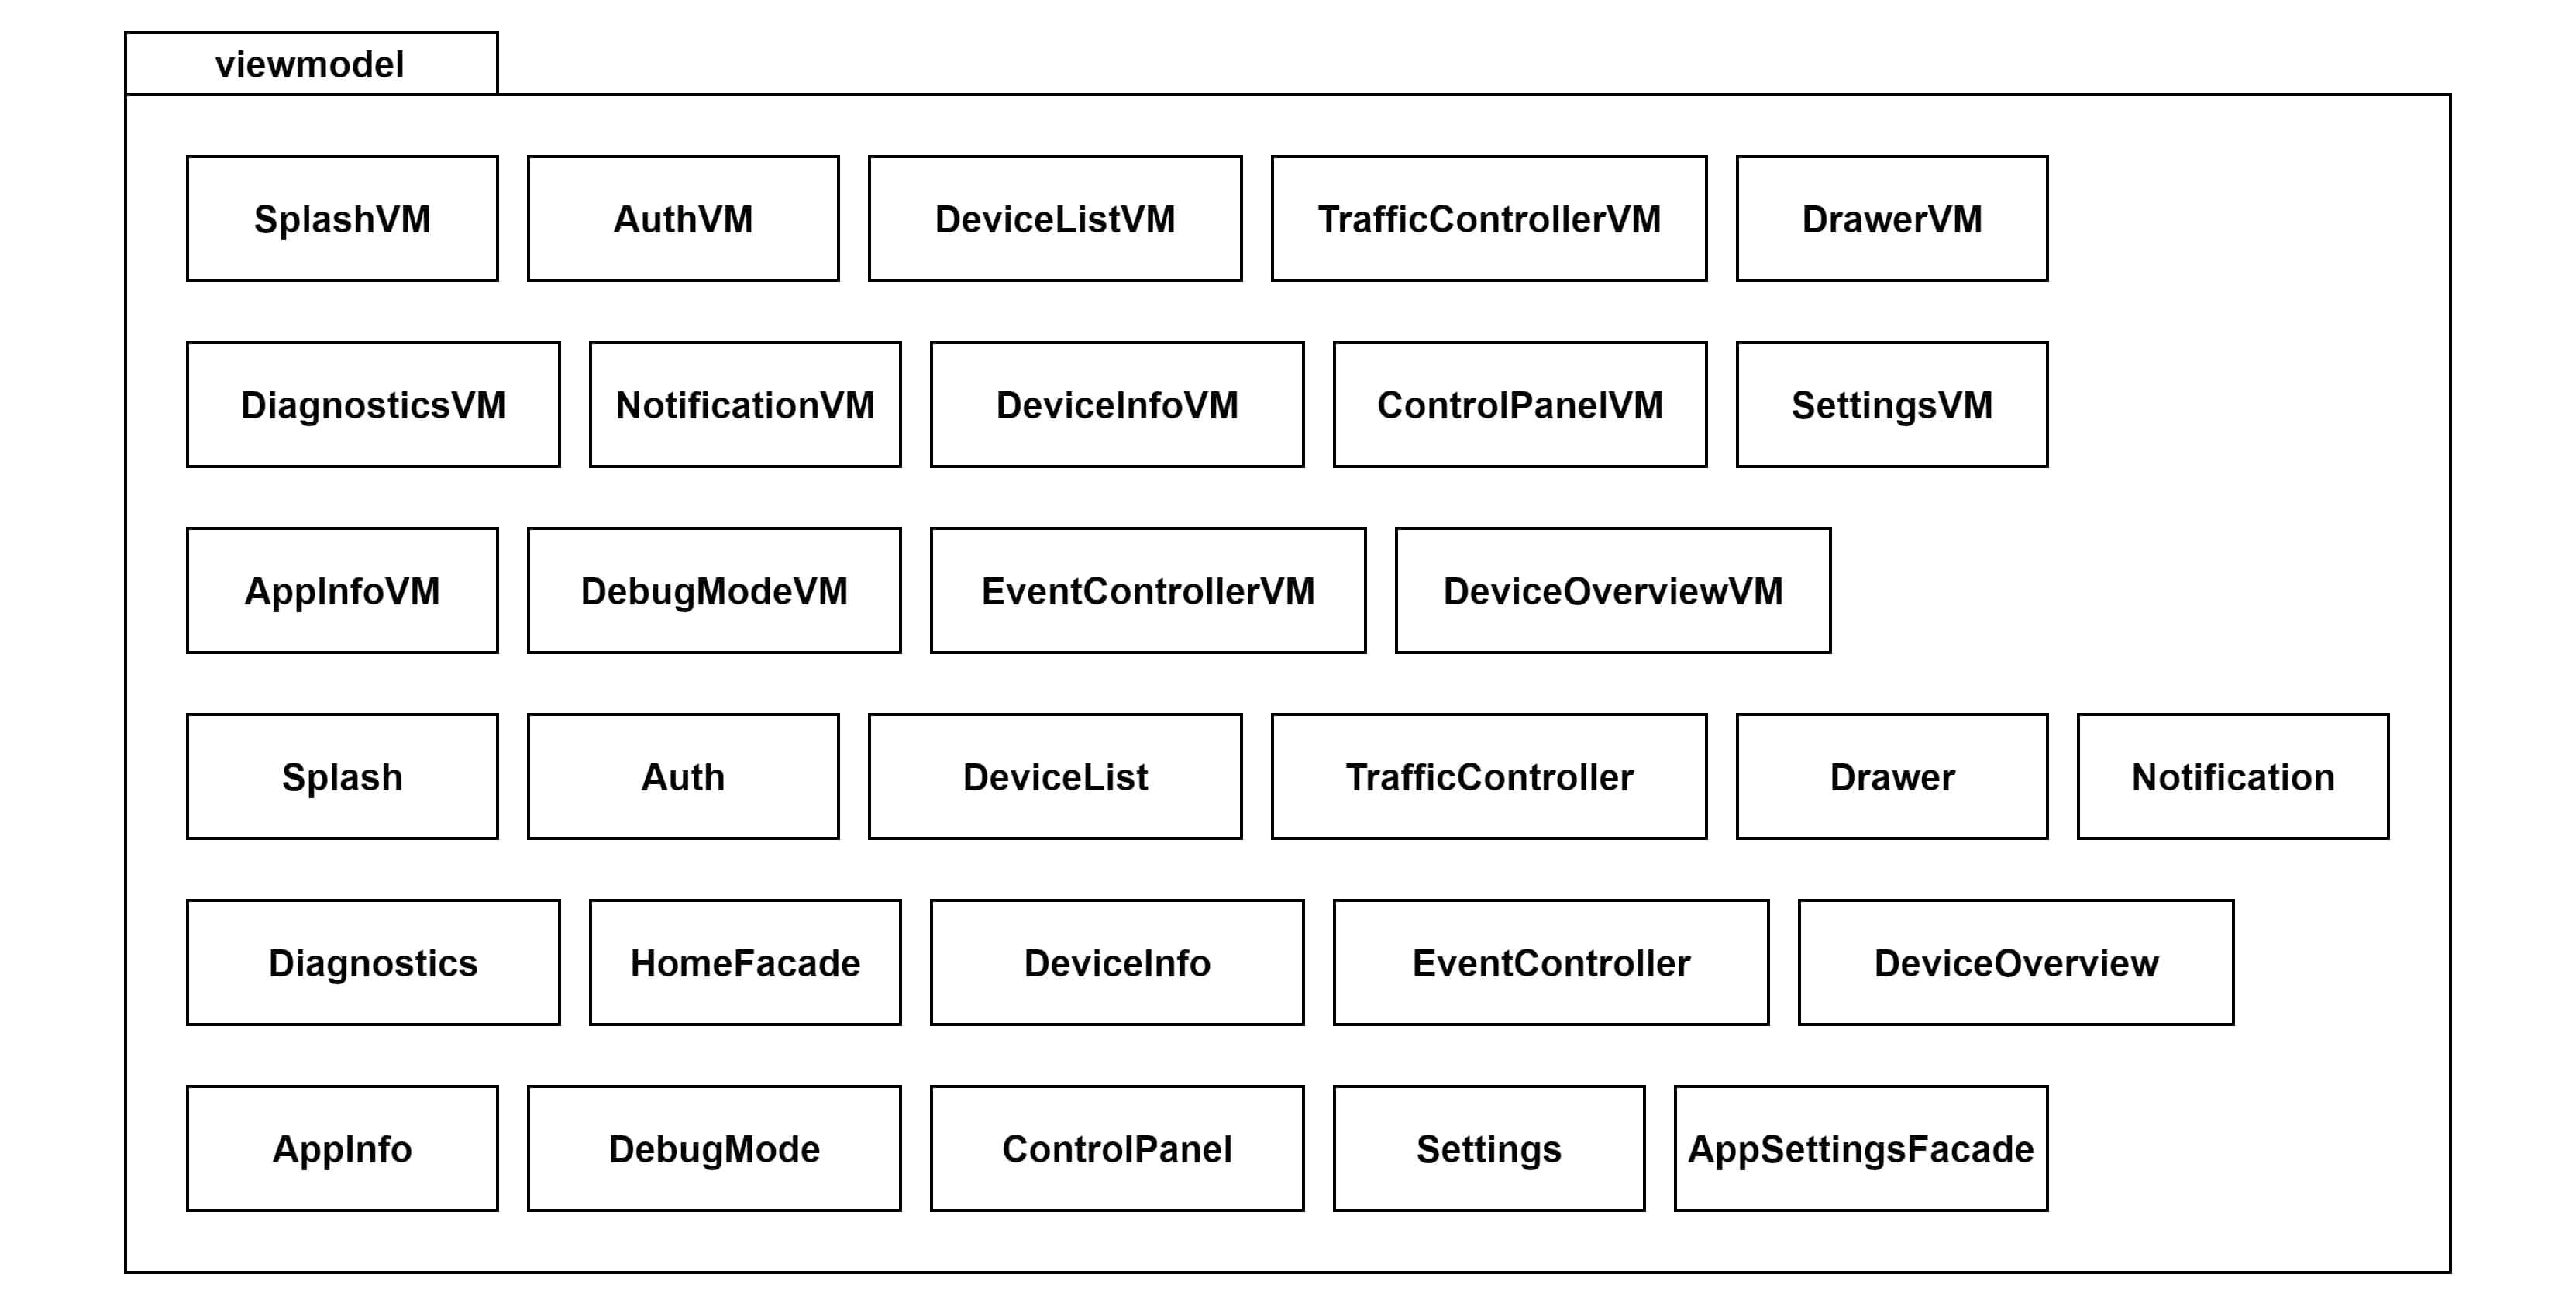
\includegraphics[width=1.0\columnwidth]{capitolo-6/organizzazione-package/viewmodel} 
  \caption{Diagramma del package \texttt{it.tecsen.smacs.viewmodel}}
\end{figure}
In questo package vi sono tutte le classi che implementano i viewmodel (ossia i model per le view) che permettono alle classi del package \texttt{view} di mostrare agevolmente i dati a schermo.\\
Per ogni viewmodel esiste un'interfaccia\footnote{Da qui in avanti in questa sezione, quando si utilizza il termine "interfaccia", si intende una classe astratta con tutti metodi astratti. Viene usato quindi il significato tipico di Java e non quello di Dart.} (tutte le classi che terminano con VM) e un'implementazione (le altre rimanenti).\\
Le classi \texttt{HomeFacade} e \texttt{AppSettingsFacade} non sono implementazioni di interfacce. Entrambi, come suggerisce il loro nome (\emph{facade}), sono classi che implementano l'omonimo \gls{designpatterng} per raggruppare funzionalità comuni necessarie alle classi del package \texttt{view}.
Il primo implementa funzionalità comuni per \texttt{SplashView} e \texttt{AuthView}. Il secondo contiene metodi e proprietà per la gestione delle impostazioni dell'applicazione, tra cui la presenza o meno di notifiche, lo stato del task in background e la durata del suo timeout di accensione.\\
Ogni interfaccia di questo package viene usata da una sola classe del package \texttt{view}, e queste non hanno accesso all'implementazione concreta. I \emph{facade} vengono invece usati in più classi dello stesso package.


%**************************************************************
\subsubsection{Package it.tecsen.smacs.utils}
\label{subsubsec:it-tecsen-smacs-utils}

\begin{figure}[!h]
  \centering 
  
\includegraphics[width=1.0\columnwidth]{capitolo-6/organizzazione-package/utils} 
  \caption{Diagramma del package \texttt{it.tecsen.smacs.utils}}
\end{figure}
In questi package ci sono strumenti di utilità creati per evitare di duplicare quanto più possibile codice.\\
Ogni classe ha il suo scopo, riassunto di seguito:
\begin{itemize}
  \item \texttt{CryptoUtils} include metodi per la cifratura di stringhe;
  \item \texttt{DateUtils} include metodi per ottenere date formattate in più modi;
  \item \texttt{FileIO} è un \emph{mixin} che viene utilizzato per memorizzare su file alcuni dati dell'applicazione dalle classi del package \texttt{it.tecsen.smacs.model.repository};
  \item \texttt{UuidUtils} include metodi per la codifica e la decodifica di \gls{uuid};
  \item \texttt{FutureUtils} include metodi per l'esecuzione sicura di funzioni che ritornano istanze di tipo \texttt{Future};
  \item \texttt{SynopticUtils} include metodi per la codifica e la decodifica di dati ottenuti dalle \gls{restg} per la visualizzazione dei dati del sinottico (casi d'uso UC04 e UC05);
  \item \texttt{UiUtils} include metodi di utilità generici per la creazione dell'interfaccia grafica.
\end{itemize}

%**************************************************************
\subsubsection{Package it.tecsen.smacs.model}
\label{subsubsec:it-tecsen-smacs-model}

\begin{figure}[!h]
  \centering 
  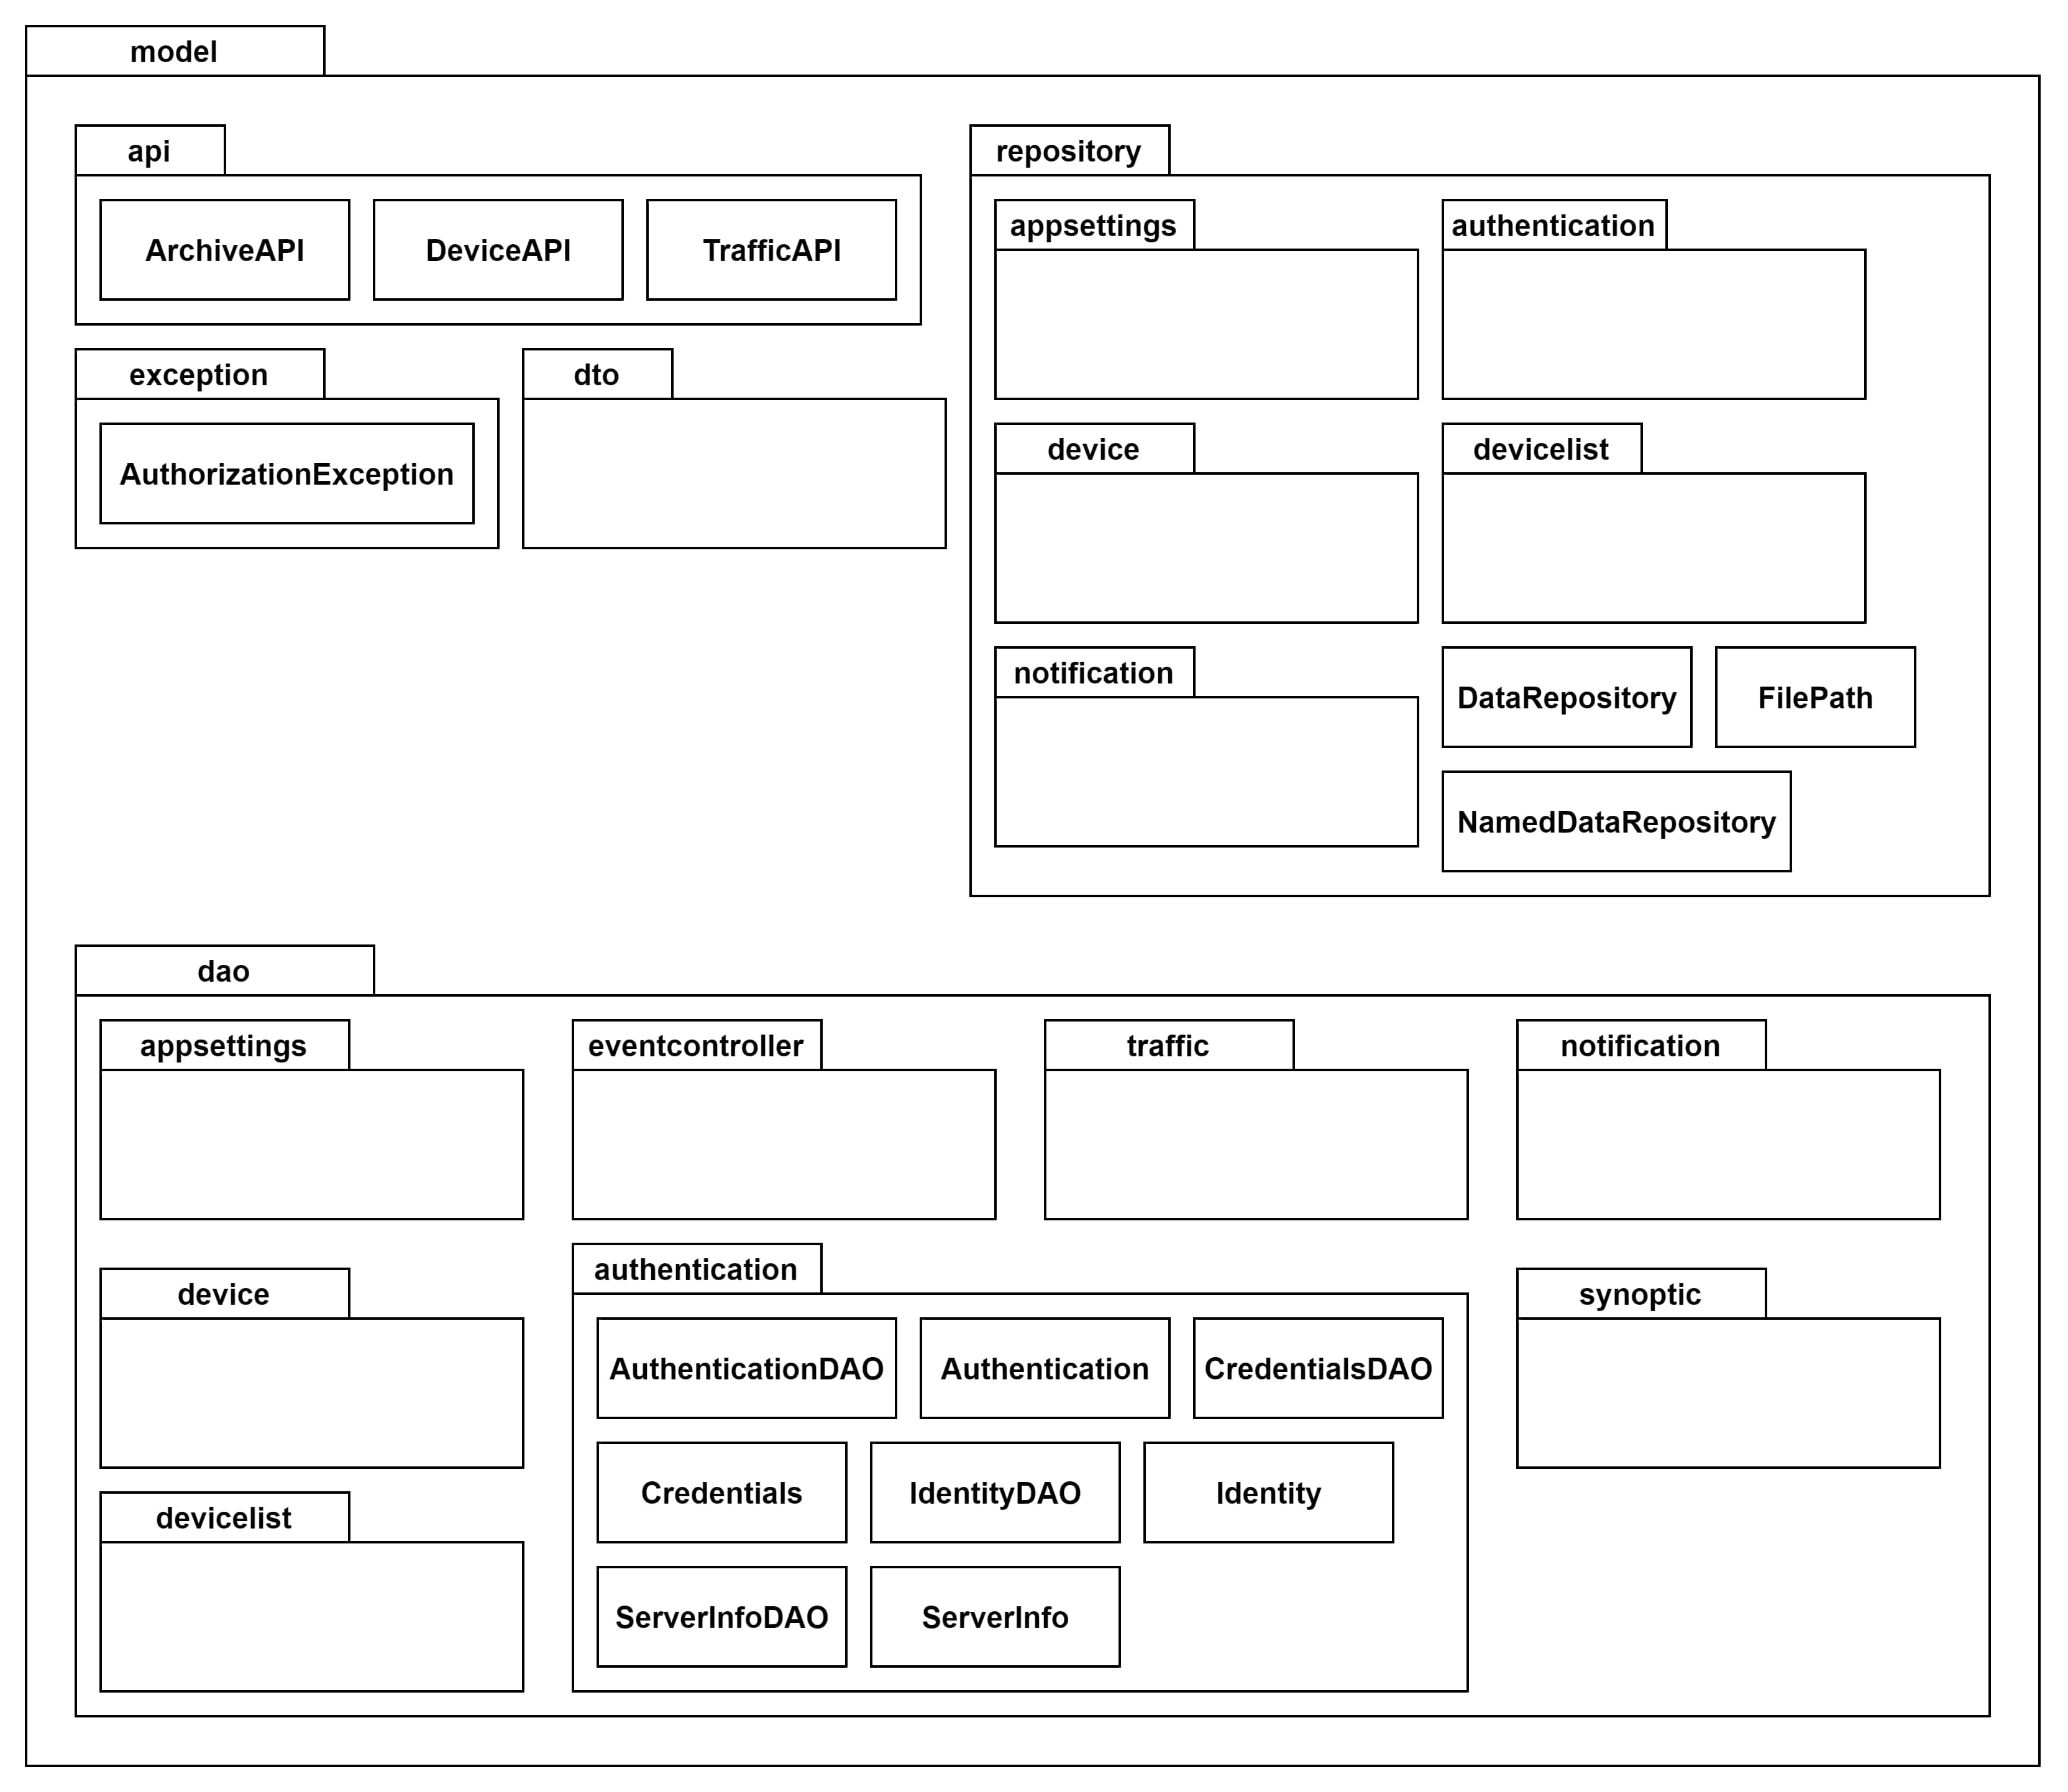
\includegraphics[width=1.0\columnwidth]{capitolo-6/organizzazione-package/model} 
  \caption{Diagramma del package \texttt{it.tecsen.smacs.model}}
\end{figure}
Questo package implementa il modello dell'applicazione.\\
Si può dividere in più aree con compiti specifici, rappresentate dai sotto-package:
\begin{itemize}
  \item \texttt{api} contiene classi che utilizzano il wrapper del package \texttt{webserviceclient} per interrogare le \gls{restg} e ritornare il risultato sotto forma di \gls{dto};
  \item \texttt{exception} contiene eccezioni che possono essere generate dalle classi presenti in questo package;
  \item \texttt{repository} contiene interfacce e classi per memorizzare su supporto persistente (le implementazioni usano dei file come supporto persistente) i dati ricevuti dai \gls{dao};
  \item \texttt{dao} contiene tutti le classi \gls{dao} che sono necessarie ai membri del package \texttt{viewmodel} per funzionare. Utilizza i package \texttt{api} e \texttt{repository} per ottenere i dati da ritornare sotto forma di \gls{dto};
  \item \texttt{dto} contiene tutti le classi \gls{dto} che sono necessarie al funzionamento dei package \texttt{api}, \texttt{dao} e \texttt{viewmodel}.
\end{itemize}
Sebbene \texttt{api} e \texttt{dao} ritornino entrambi \gls{dto}, c'è una differenza:
\begin{itemize}
  \item il primo non fa nessuna elaborazione sui dati, semplicemente li ottiene dalle \gls{restg} sotto forma di \gls{json}, ne fa il parsing e restituisce quanto ottenuto;
  \item il secondo elabora i \gls{dto} ottenuti dal primo e li ritorna elaborati (per fare un esempio, una lista ricevuta da \texttt{api} potrebbe essere ordinata, filtrata e poi ritornata).
\end{itemize}

%**************************************************************
\subsubsection{Package it.tecsen.smacs.webserviceclient}
\label{subsubsubsec:it-tecsen-smacs-webserviceclient}

\begin{figure}[!h]
  \centering 
  
\includegraphics[width=1.0\columnwidth]{capitolo-6/organizzazione-package/webserviceclient} 
  \caption{Diagramma del package \texttt{it.tecsen.smacs.webserviceclient}}
\end{figure}
In questo package vi sono tutte le classi che implementano il wrapper della libreria \emph{http}, come è stato precedentemente illustrato in "\hyperref[subsubsec:it-tecsen-smacs]{Package it.tecsen.smacs}".


%**************************************************************
\subsubsection{Package it.tecsen.smacs.widget}
\label{subsubsubsec:it-tecsen-smacs-widget}

Il package \texttt{widget} non è stato riportato sotto forma diagrammatica per due ragioni:
\begin{itemize}
  \item perché è troppo vasto e dispersivo;
  \item perché contiene solo classi il cui scopo è permettere quanto più riuso di codice possibile per la parte di interfaccia utente.
\end{itemize}

%**************************************************************
\subsubsection{Package it.tecsen.smacs.config}
\label{subsubsubsec:it-tecsen-smacs-config}

Il package \texttt{config} non è stato riportato sotto forma diagrammatica perché come indicato in in "\hyperref[subsubsec:it-tecsen-smacs]{Package it.tecsen.smacs}" contiene principalmente configurazioni per il funzionamento di altre classi.

%**************************************************************
\subsection{Il design pattern Observer: Provider, ChangeNotifier e Consumer}
\label{subsec:observer-provider-changenotifier}

È stato detto che una delle caratteristiche dell'architettura MVVM è la presenza di un doppio Observer.\\
L'Observer è un \gls{designpatterng} formalizzato dalla "Gang of Four" nel libro \emph{Design Patterns - Elementi per il riuso di software ad oggetti}.\\
Permette:
\begin{itemize}
  \item di avere dipendenze di tipo "1 a molti" fra oggetti, permettendo di avere consistenza in maniera agevole;
  \item divide gli oggetti possessori di stato nella categoria \emph{Subject} e quelli che dipendono da questo stato in \emph{Observer};
  \item quando un \emph{Subject} aggiorna il suo stato notifica i propri \emph{Observer} (internamente dispone di un riferimento per ciascuno di questi, ma non sa nulla di loro per via dell'astrazione).
\end{itemize}
Di seguito viene presentato un esempio per illustrare come è stato implementato il \gls{designpatterng} Observer all'interno del prodotto.
L'esempio si riferisce alla parte del sistema in cui un \emph{ViewModel} ha ricevuto dai \gls{dao} da cui dipende una nuova lista e quindi notifica qualsiasi \emph{View} in ascolto.
Solo alcune parti (quelle fondamentali ai fini dell'esempio) vengono riportate.

%**************************************************************
\subsubsection{Il Subject: ChangeNotifier}
\label{subsubsec:subject-changenotifier}

In \emph{Flutter} (e non Dart, perché è propriamente una caratteristica del \gls{frameworkg}) un \emph{Subject} è realizzabile molto semplicemente aggiungendo nella firma di una classe il mixin \texttt{ChangeNotifier}, come mostrato di seguito:

\begin{lstlisting}
class DeviceList with ChangeNotifier implements DeviceListVM {
  ...

  DeviceListDAO _deviceListDAO;
  
  ...
}
\end{lstlisting}
In questa porzione di classe sono messi in vista anche \texttt{DeviceListVM}, che è la dipendenza di cui necessita la \emph{View} e \texttt{DeviceListDAO} che è invece una dipendenza di questo \emph{ViewModel}.\\
Nel metodo in cui viene aggiornato lo stato avviene anche la notifica degli \emph{Observer}:
\begin{lstlisting}
@override
Future<void> syncDeviceList({final bool forceDownload = false}) async {
    ...

    await _deviceListDAO.syncDeviceList(_token, _deviceTree, forceDownload: forceDownload);

    notifyListeners();
}
\end{lstlisting}
Come si può notare, dopo aver chiamato il metodo \texttt{syncDeviceList} di \texttt{DeviceListDAO} a riga 5, viene invocato il metodo \texttt{notifyListeners} che appartiene al \emph{mixin} \texttt{ChangeNotifier}.\\
Una volta ricevuta la notifica, uno dei primi metodi che viene richiamato dalla vista è quello che ritorna la cardinalità della lista che è appena stata scaricata (successivamente seguono altre chiamate), in base alla selezione dell'utente:
\begin{lstlisting}
@override
Future<int> get selectedDeviceListLength async {
  List<Device> devices;

  if (_activeDisplayMode == DisplayMode.ALPHABETICAL_ORDER) {
    devices = _deviceListDAO.alphabeticalOrderDeviceList;
  } else {
    devices = _deviceListDAO.warningDeviceList;
  }

  if (_nearbyDevicesMode) {
    devices = await _deviceListDAO.nearbyDeviceList(deviceList);
  }

  return devices.length;
}
\end{lstlisting}
I due costrutti \texttt{if} servono a verificare che tipo di lista va ritornata all'utente (in base alle sue precedenti selezioni), per invocare il metodo corretto.

%**************************************************************
\subsubsection{Il Subject: Provider}
\label{subsubsec:subject-provider}

Come è stato già illustrato al capitolo 5 sulla "\hyperref[cap:dependency-injection]{Dependency Injection}", un'istanza di \texttt{DeviceListVM} va messa a disposizione dei widget figli attraverso un \emph{Provider} come antenato nel \emph{Widget tree}.\\
In questo caso, visto che \texttt{DeviceListVM} usa \texttt{ChangeNotifier} ed ha delle dipendenze esterne (due, per l'esattezza), viene istanziato un \texttt{ChangeNotifierProxyProvider2}.
\begin{lstlisting}
class DeviceListScreen extends StatelessWidget {
  ...

  @override
  Widget build(BuildContext context) {
    return ChangeNotifierProxyProvider2<IdentityDAO, DeviceListDAO, DeviceListVM>(
      // Viene creata l'istanza ma non viene usata 
      // (non ha i riferimenti ai DAO).
      create: (_) => DeviceList(),
      // Viene aggiornata l'istanza con i nuovi DAO.
      update: (_, identityDao, deviceListDao, deviceListVM) {
        deviceListVM.deviceListDAO = deviceListDao;
        deviceListVM.identityDAO = identityDao;
        return deviceListVM;
      },

      ...
    );
  }
}
\end{lstlisting}
In \texttt{ChangeNotifierProxyProvider2} il parametro \texttt{update} gestisce il caso in cui le dipendenze di \texttt{DeviceListVM} chiamino anche loro \texttt{notifyListeners}.

%**************************************************************
\subsubsection{L'Observer: Consumer}
\label{subsubsec:observer-consumer}

Un altro modo per chiamare il \gls{designpatterng} Observer è "Producer-Consumer", in cui il \emph{Producer} corrisponde al \emph{Subject} e l'\emph{Observer} corrisponde al \emph{Consumer}.\\
Senza troppa fantasia, un widget che in \emph{Flutter} si occupa di agire da \emph{Consumer} ha proprio questo nome: si registra come \emph{Observer} rispetto ad un \emph{ChangeNotifier} e ogni volta che riceve una notifica ricostruisce il suo sotto albero (la porzione di \emph{Widget tree} radicata nel suo primo discendente).
% Extra a capo per arrivare a fine pagina
\clearpage

\begin{lstlisting}
class DeviceListScreen extends StatelessWidget {
  ...

  @override
  Widget build(BuildContext context) {
    ...
  
    return ChangeNotifierProxyProvider2<IdentityDAO, DeviceListDAO, DeviceListVM>(
      child: Consumer<DeviceListVM>(
        // Il terzo parametro, noRedraw, corrisponde ad un widget che non va ricostruito nel caso DeviceListVM emetta notifiche.
        builder: (_, deviceListVM, noRedraw) {
          return ScreenViewSafeContainer(
            child: DeviceListView(),
            bottomAppBar: FutureBuilder<int>(
            future: deviceListVM.selectedDeviceListLength,
            ...
          );
        }
        ...
      ),
    );
  }
}
\end{lstlisting}
Come si può notare si è continuato l'esempio di prima (è la stessa classe e lo stesso metodo \texttt{build}).\\
Come affermato poc'anzi, ad ogni \texttt{notifyListeners} invocato da \texttt{DeviceListVM}, verrà ricostruito il sottoalbero radicato nel primo discendente disponibile del widget \texttt{Consumer}, ovvero \texttt{ScreenViewSafeContainer} (propriamente viene invocato nuovamente il \emph{callback} \texttt{builder} a riga 11, ma è un dettaglio del \gls{frameworkg} che non cambia il principio di funzionamento).

%**************************************************************
\section{Confronto fra la precedente app e quella nuova}
\label{sec:confronto-precedente-app-nuova}

In questa sezione vengono mostrate le differenze più significative fra la precedente app (in uso presso l'azienda) e quella nuova, realizzata durante lo stage.\\
Queste differenze sono dovute principalmente alla richiesta da parte del tutor aziendale di pensare a come poter fare un restyling grafico dell'applicazione che attualmente hanno in uso.
Quest'ultima infatti, essendo un po' datata, è stata progettata con un impianto grafico e con un'esperienza utente diverse da quelle da quelle attuali.\\
Innanzitutto, gli schermi degli smartphone e dei tablet sono, negli ultimi anni, diventati sempre più grandi e con risoluzioni più elevate, offrendo più spazio per disporre il contenuto di una schermata.
Non ha quindi più senso, ad esempio, avere liste scorrevoli di elementi che sono condensate. Ci si può permettere di spaziare molto di più gli elementi e anche migliorare anche lo spazio fra una linea di testo e un'altra.\\
Inoltre, entrambi i sistemi operativi per cui sviluppare l'applicazione hanno un loro stile grafico, per cui va valutato se creare due interfacce utenti del tutto simili ma con componenti che ricalcano quelle native oppure cercare di creare un'interfaccia che possa andare bene per entrambe, evitando di utilizzare componenti grafiche specifiche per l'uno o per l'altro sistema.
Ad esempio, nel \emph{Material Design} di Google vi sono delle componenti chiamate \emph{Floating Action Button} (dei pulsanti a forma circolare posizionati solitamente in basso al centro/destra che "fluttuano" sopra il contenuto), da utilizzare come pulsanti per svolgere azioni come la modifica di contenuti testuali, che in Android si integrerebbero correttamente, in iOS invece no.\\
Un'altra riflessione che è stata fatta è relativa ai menu principale dell'applicazione: come viene mostrato in "\hyperref[subsec:menu-applicazione]{Menu dell'applicazione}", difficilmente viene ancora usato un menu a tendina per mostrare funzionalità secondarie, preferendo invece un menu di tipo "drawer".\\
Altre considerazioni e dimostrazione dei miglioramenti apportati si possono trovare nelle sotto-sezioni che seguono.

% \clearpage % Tenere se non viene scritto altro in questa sezione.

%**************************************************************
\subsection{Informazioni sull'applicazione}
\label{subsec:informazioni-applicazione}

Questa schermata è disponibile aprendo il menu dell'applicazione (schermata che viene presentata in seguito a questa) e mostra informazioni generali sull'applicazione, tra cui il server a cui si è connessi, il nome utente e la versione.\\
Il contenuto di questa schermata, che nella app dell'azienda è condensato verso l'alto, viene ora reso più spaziato e inserito in più elementi di una lista scorrevole permettendo, in futuro, di aggiungere contenuti alla schermata senza problemi.\\
I due loghi, dell'azienda presso cui si è svolto lo stage e dell'azienda di cui è partner, sono stati resi cliccabili ed entrambi reindirizzano al rispettivo sito web.

\begin{figure}[!h]
  \centering 
  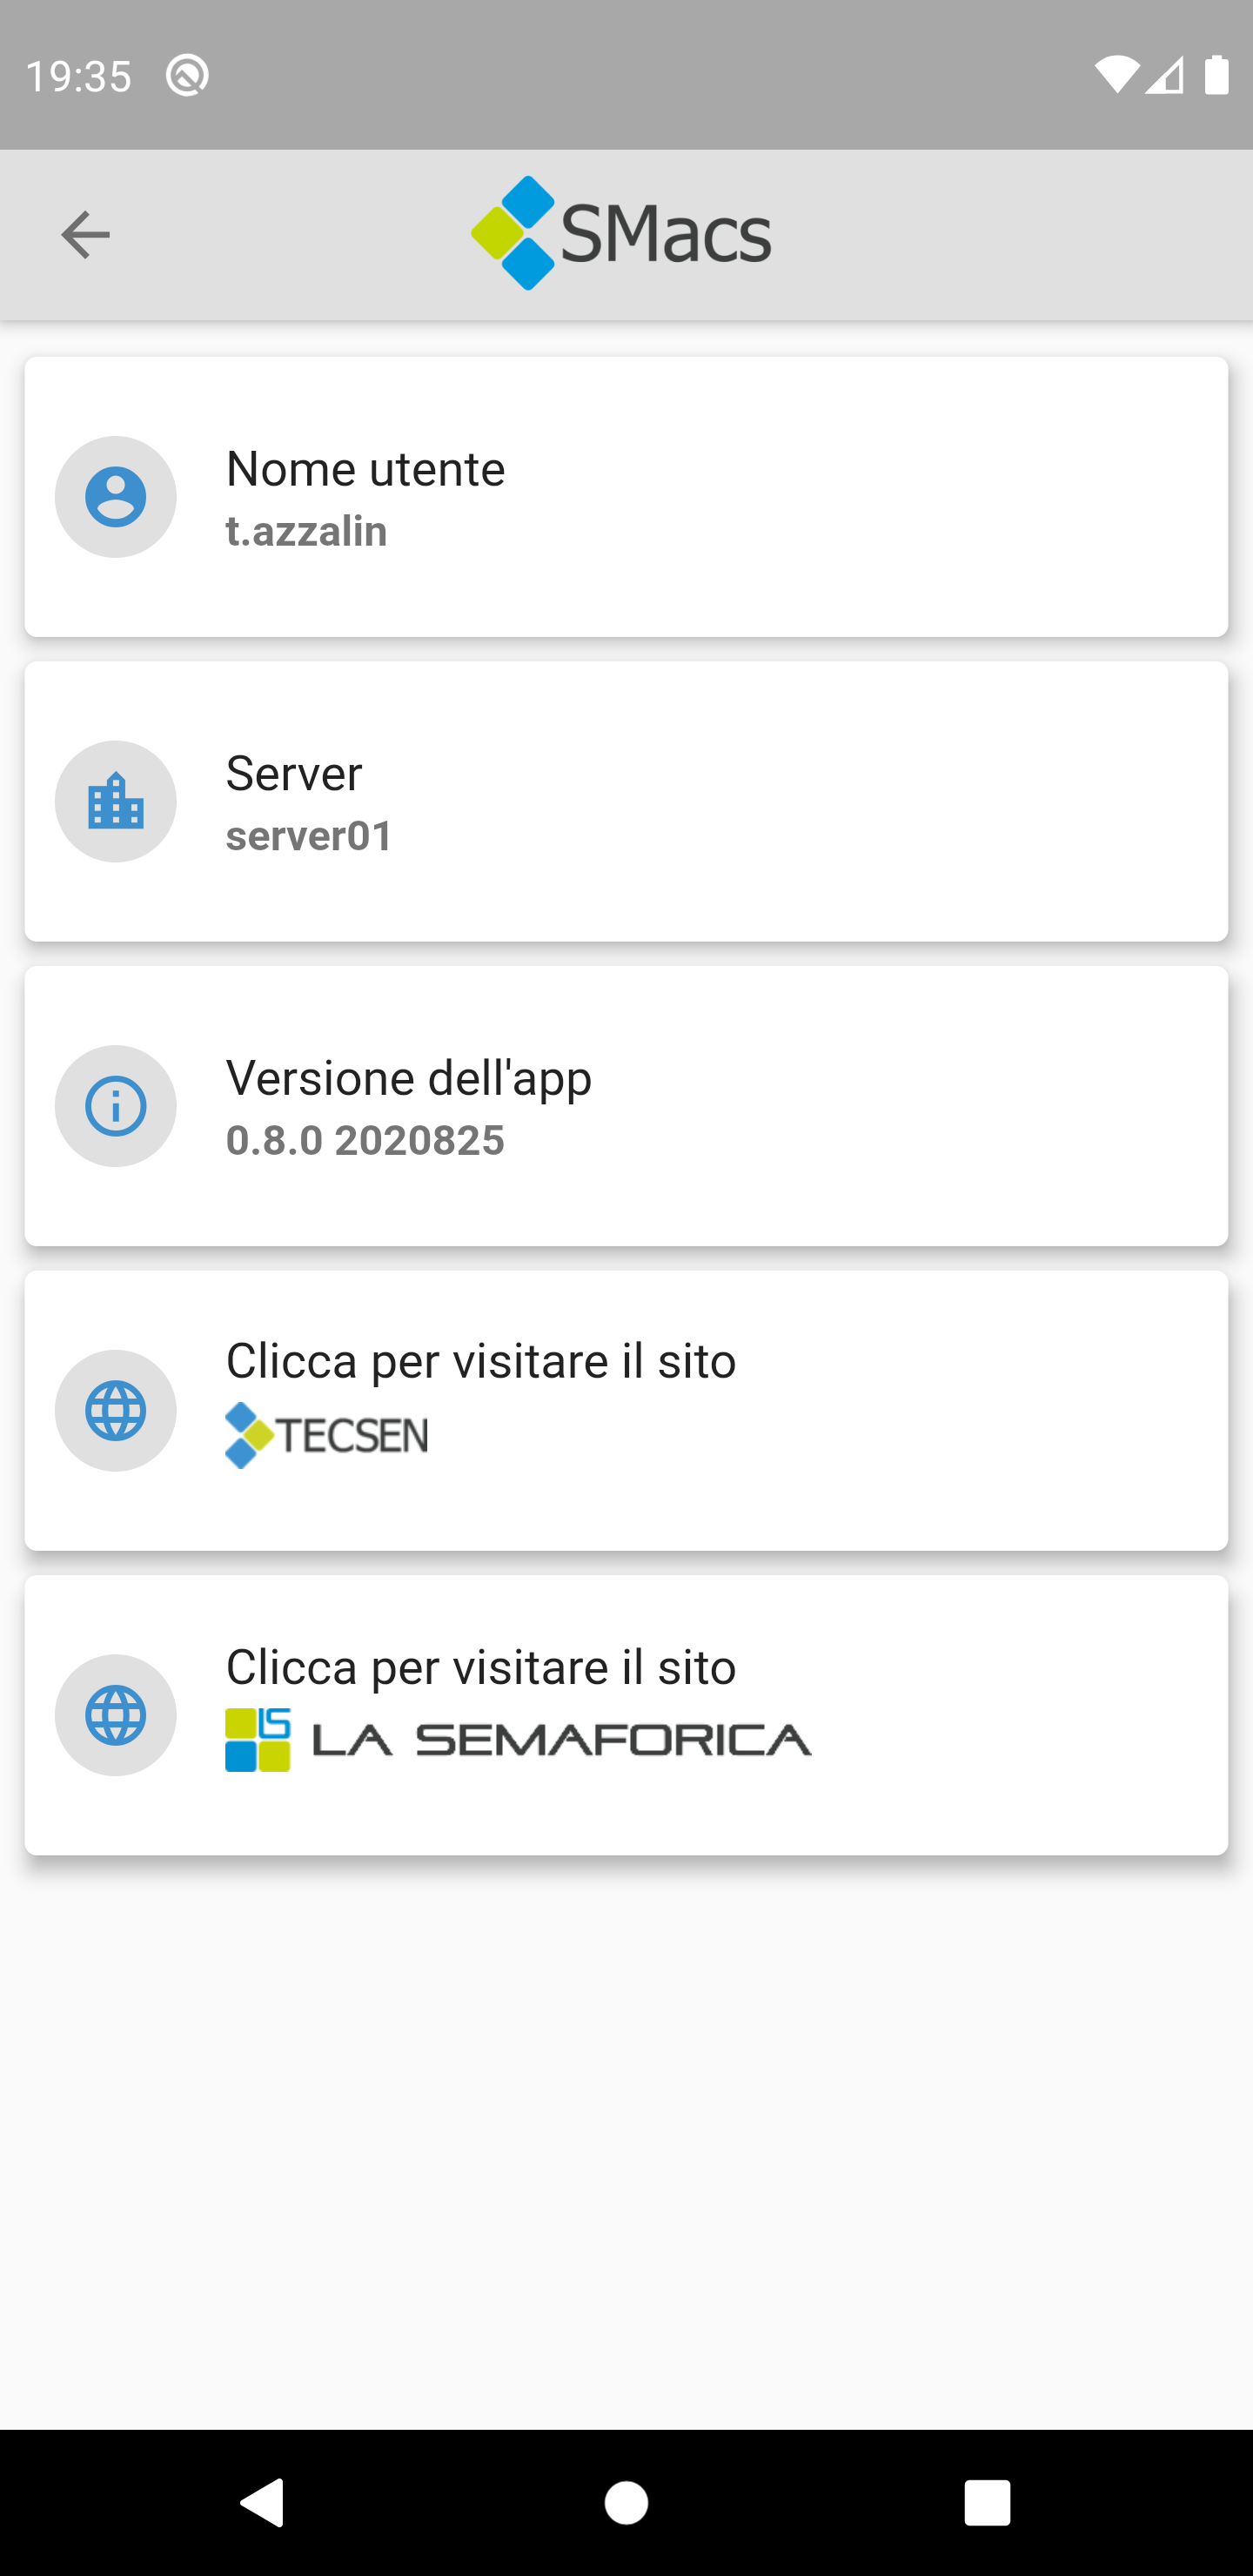
\includegraphics[width=0.75\columnwidth]{capitolo-6/confronto-app-vecchia-nuova/AppInfoView} 
  \caption{Confronto fra schermate delle app: Informazioni sull'applicazione}
\end{figure}

\clearpage % Tenere per assicurarsi che ci sia un'immagine per pagina e basta.

%**************************************************************
\subsection{Menu dell'applicazione}
\label{subsec:menu-applicazione}

Il menu dell'applicazione è accessibile, così come nell'app dell'azienda, solamente attraverso la schermata della lista degli impianti.\\
Prima disponibile sotto forma di menu a tendina, nella versione realizzata per lo stage è stato realizzato un menu di tipo \emph{drawer} (dall'inglese, cassetto, perché alla richiesta di apertura effettua una transizione dall'esterno all'interno e si richiude in maniera inversa), che appare da sinistra alla pressione del pulsante \emph{hamburger} (il pulsante con tre linee parallele orizzontali è stato così ribattezzato perché assomiglia ad un panino di un fast food) in alto a sinistra (visibile nella schermata di destra nell'immagine sottostante).\\
Le voci del menu sono state mantenute così com'erano ad eccezione della voce "Refresh", che aggiorna la lista di impianti disponibile localmente riscaricandola dai server aziendali, che è stata rimossa in favore di un più accessibile pulsante presente direttamente nella barra di navigazione in alto alla schermata, riducendo il numero di click necessari per raggiungerlo.

\begin{figure}[!h]
  \centering 
  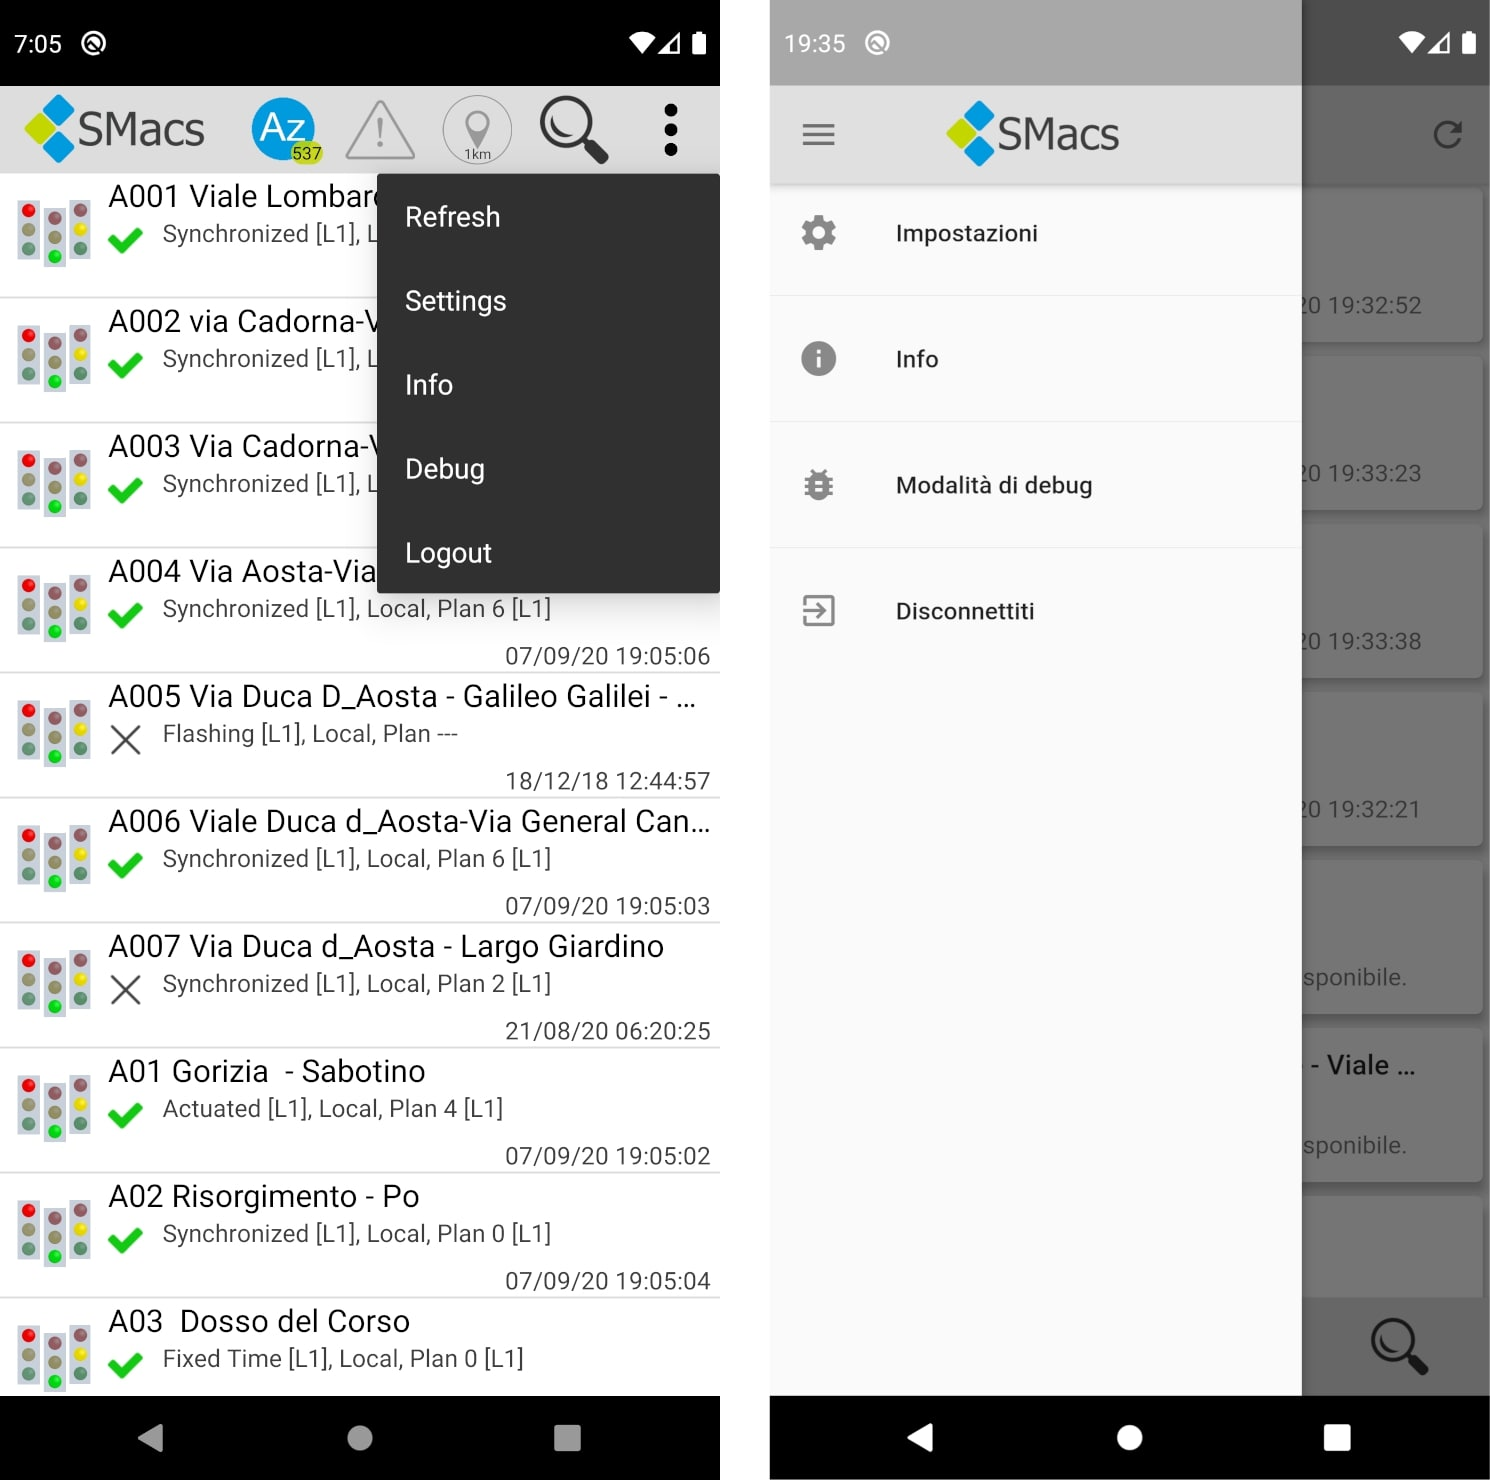
\includegraphics[width=1.0\columnwidth]{capitolo-6/confronto-app-vecchia-nuova/DrawerView} 
  \caption{Confronto fra schermate delle app: Menu dell'applicazione}
\end{figure}

\clearpage % Tenere per assicurarsi che ci sia un'immagine per pagina e basta.

%**************************************************************
\subsection{Lista degli impianti}
\label{subsec:lista-impianti}

La schermata in cui viene mostrata la lista degli impianti è rimasta sostanzialmente invariata se non per alcune modifiche prettamente estetiche.\\
I pulsanti per filtrare la lista sono stati spostati dalla barra di navigazione in alto a una barra apposita in basso e, come è stato detto in precedenza, il pulsante di "Refresh" è stato estratto dal menu per averlo disponibile nella barra di navigazione.\\
A differenza dell'applicazione in uso presso l'azienda, non tutte le funzionalità sono disponibili: tutti gli elementi della lista la cui icone rappresentano dei semafori sono cliccabili (e portano alla schermata di dettaglio) mentre gli altri, come i primi due elementi della lista della schermata di destra, non lo sono.\\
In quest'ultimo caso, la pressione dell'elemento visualizza un avviso all'utente che lo informa sul fatto che la funzionalità non è ancora disponibile.

\begin{figure}[!h]
  \centering 
  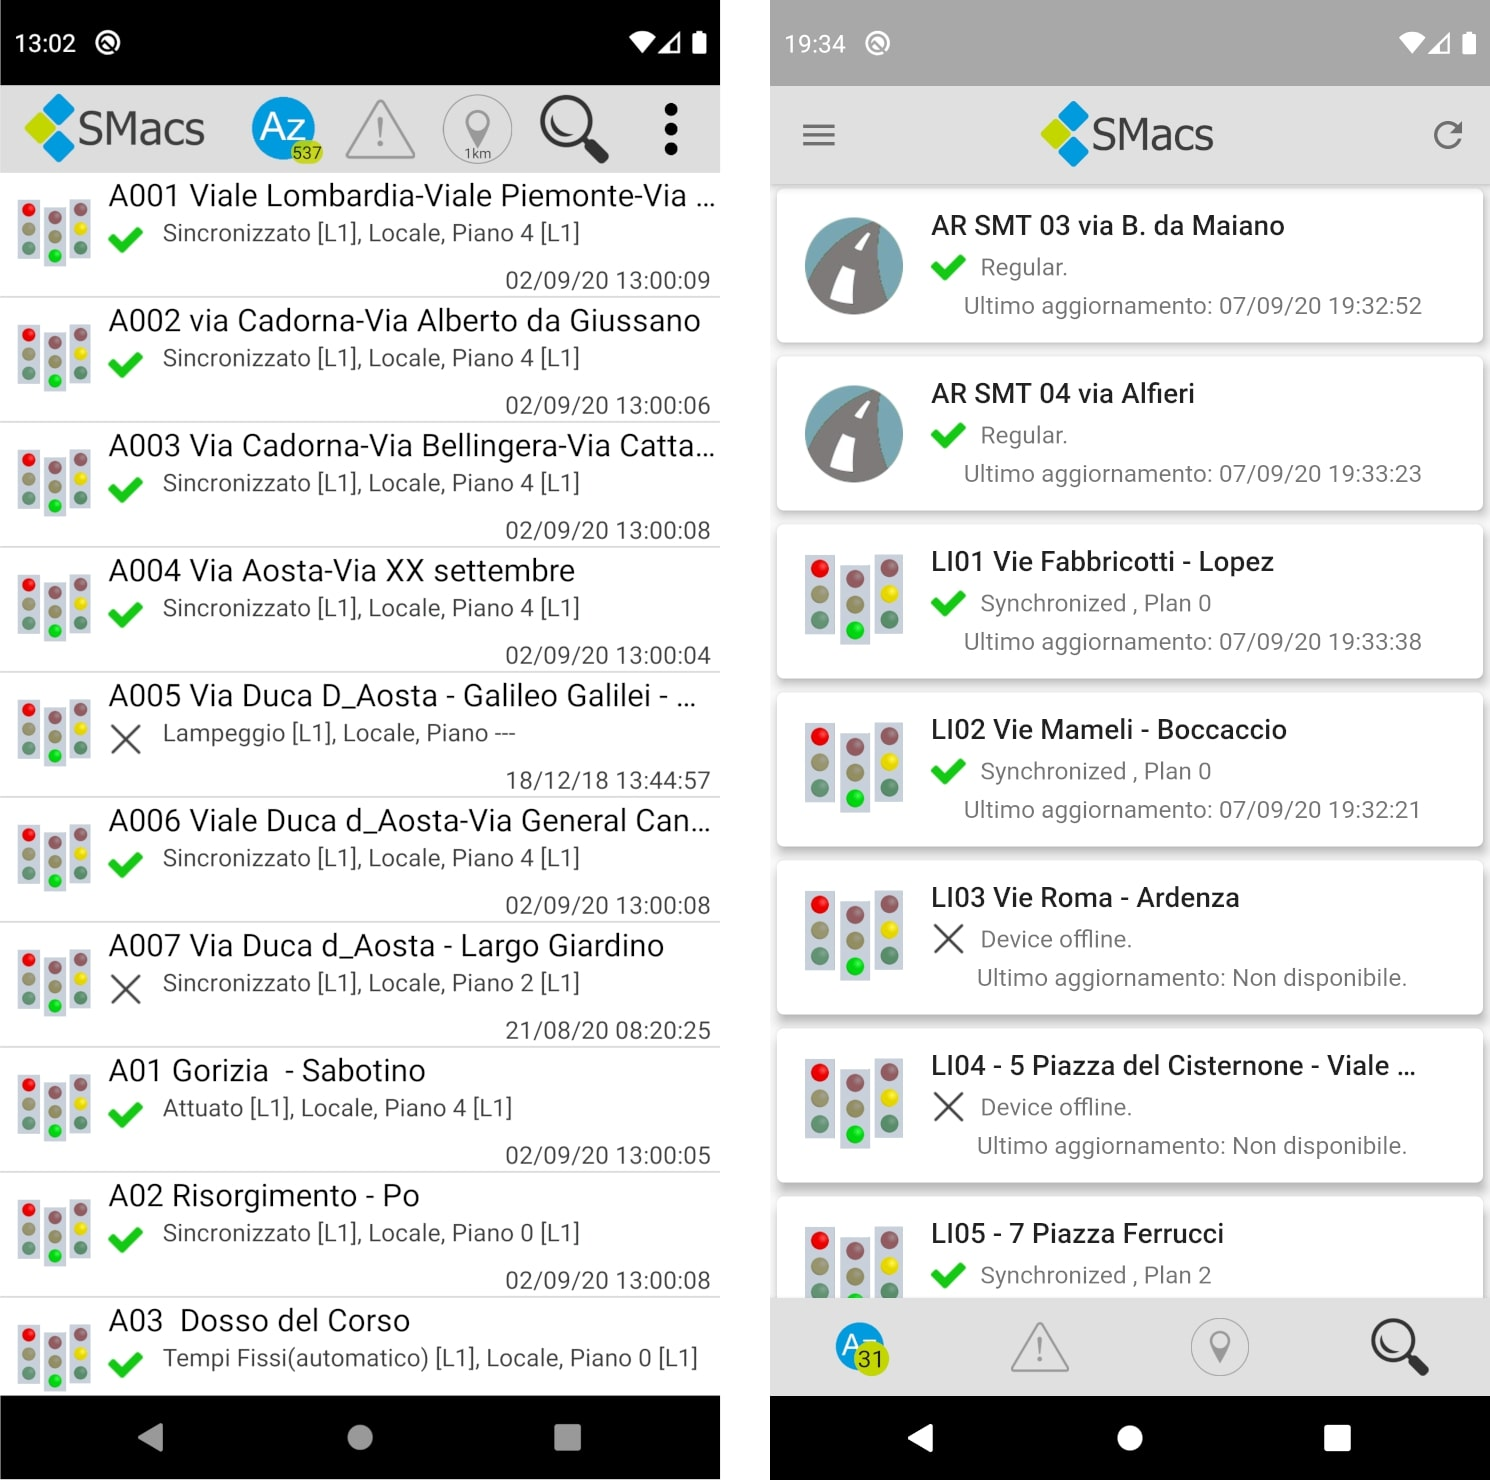
\includegraphics[width=1.0\columnwidth]{capitolo-6/confronto-app-vecchia-nuova/DeviceListView} 
  \caption{Confronto fra schermate delle app: Lista degli impianti}
\end{figure}

\clearpage % Tenere per assicurarsi che ci sia un'immagine per pagina e basta.

%**************************************************************
\subsection{Pannello di controllo}
\label{subsec:pannello-controllo}

La schermata del dettaglio di un regolatore semaforico è cambiata sensibilmente.\\
Questa schermata comprende tutta ciò che è presente nell'immagine di destra, incluse le tre schede "Panoramica", "Diagnostica", "Pannello di controllo" e il loro contenuto.
Dalla pulsantiera in basso sono stati rimossi il "Pannello di controllo", che è appunto diventata una scheda, e il pulsante "Indicazioni stradali", giustificato dal fatto che premendo il pulsante "Posizione" si apre l'applicazione di mappe del dispositivo, che già propone l'avvio nella navigazione.\\
È stato invece inserito il pulsante "Info" che rimanda alla schermata con le informazioni dell'hardware e del software del regolatore semaforico.\\
Oltre a queste modifiche, che sono comuni a "Panoramica" e a "Diagnostica", nella schermata "Pannello di controllo" è stata semplificata l'interfaccia, rendendola più simile a quella attualmente usata negli applicativi per desktop dell'azienda (a fini di unificazione dell'esperienza utente).
In particolare, la pulsantiera "Funzione" è diventata un menu a tendina, "Reset allarmi" è stata spostata nella scheda "Diagnostica" e le altre funzionalità è stato chiesto di non inserirle.

\begin{figure}[!h]
  \centering 
  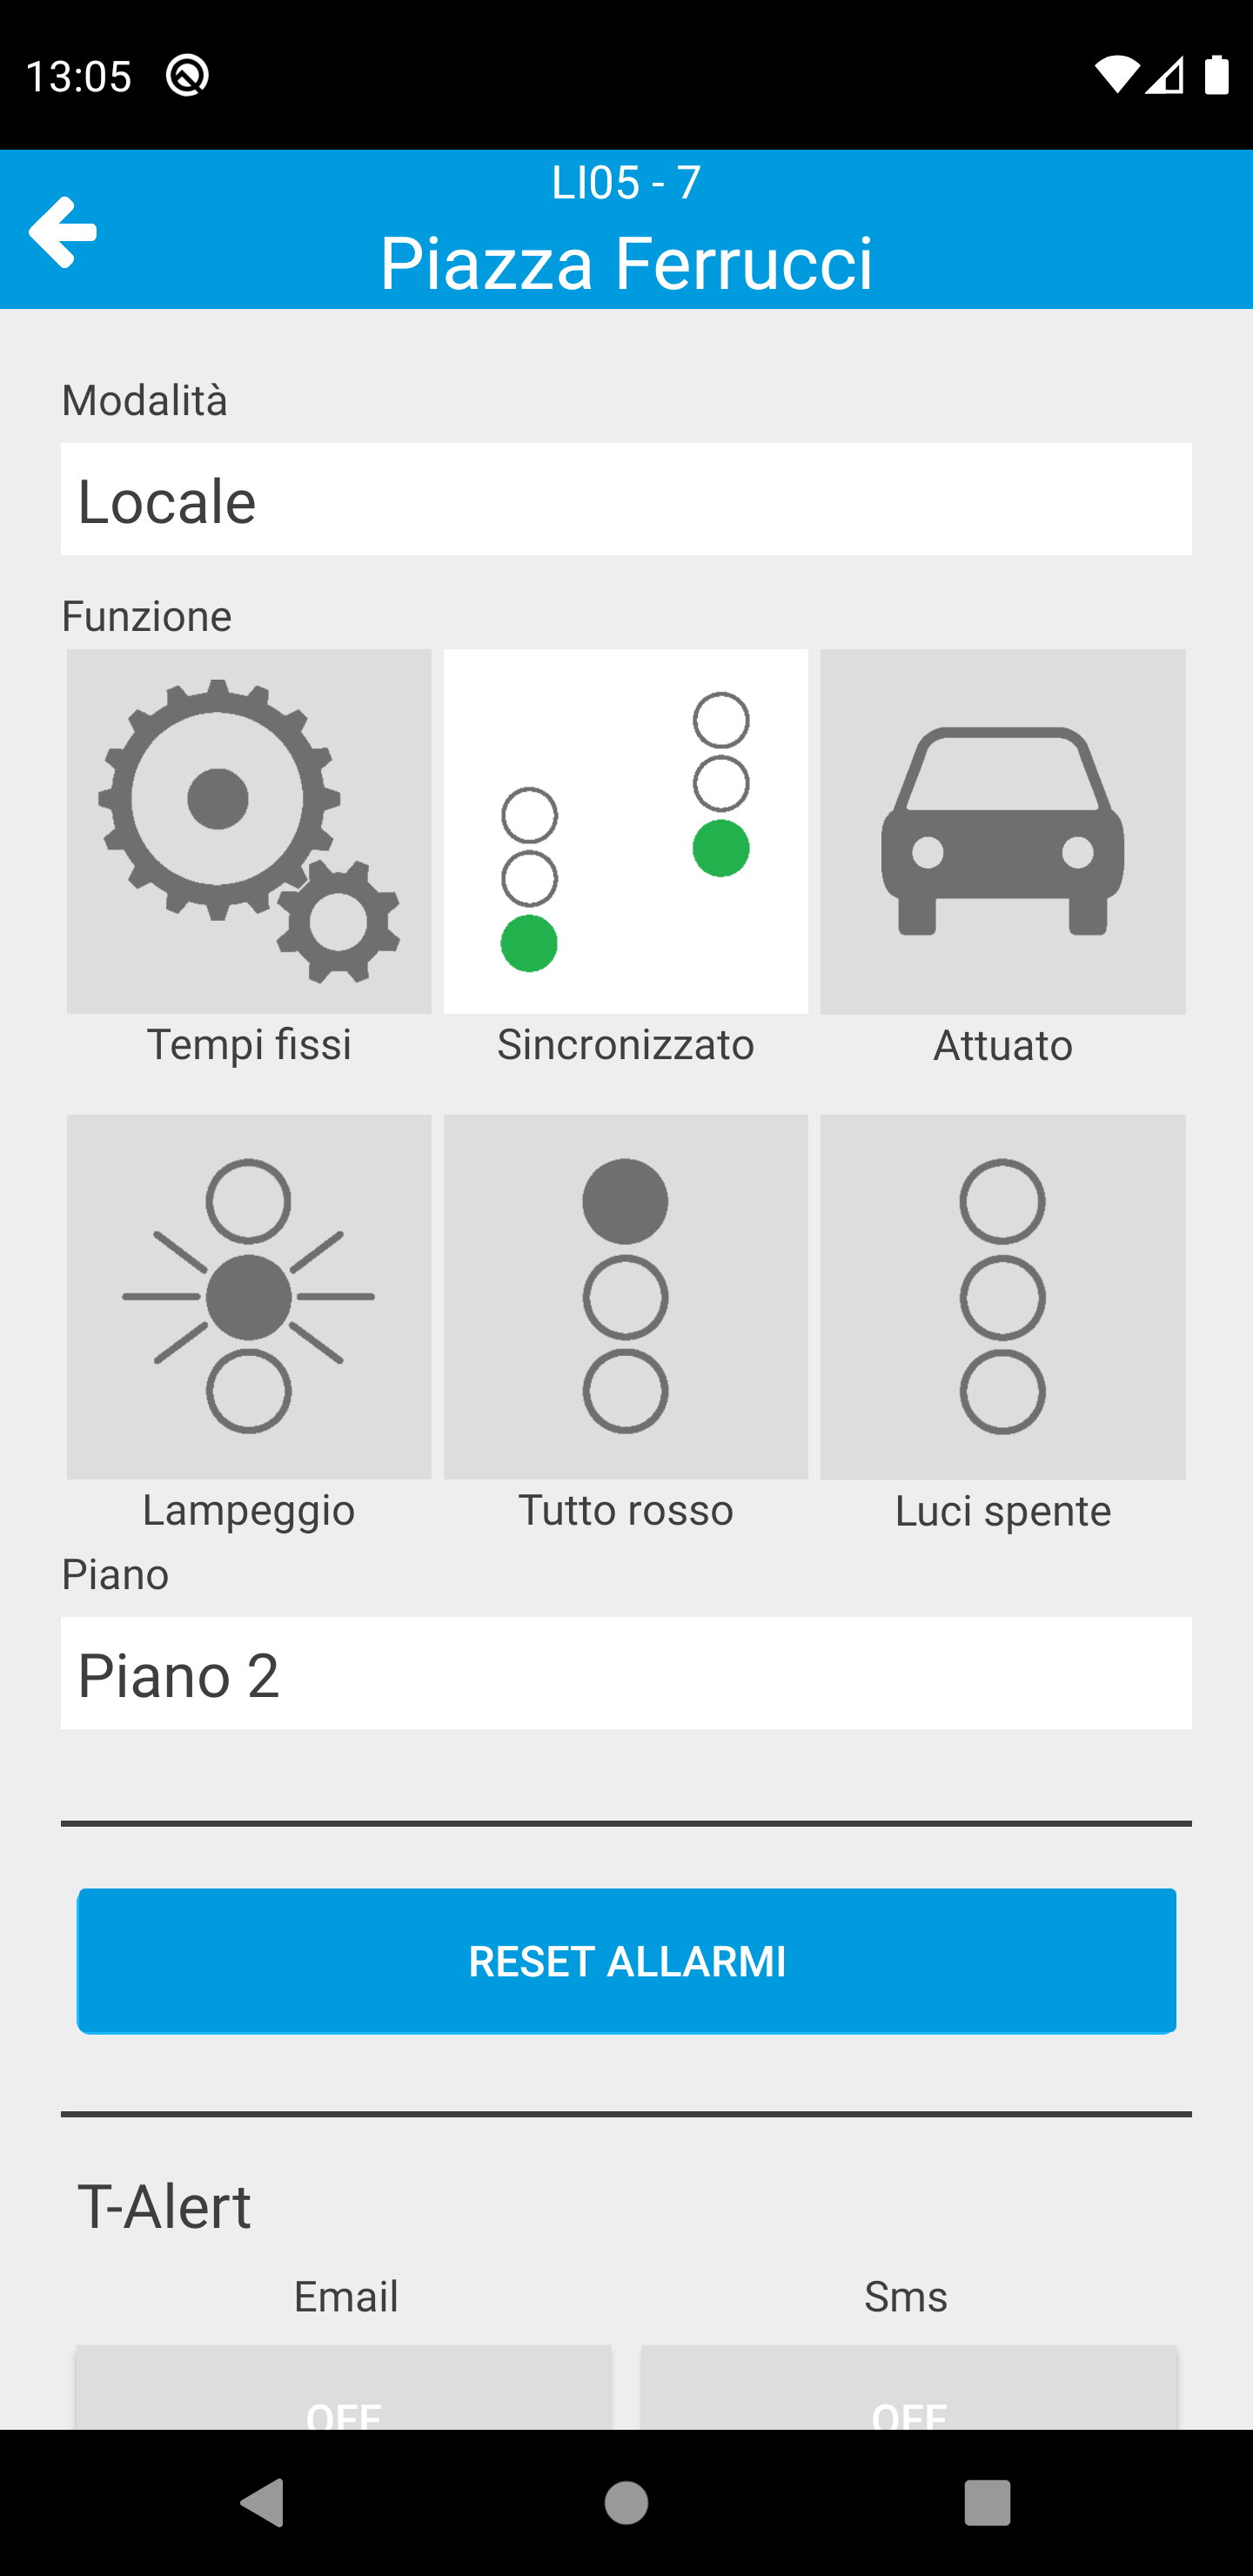
\includegraphics[width=1.0\columnwidth]{capitolo-6/confronto-app-vecchia-nuova/ControlPanelView} 
  \caption{Confronto fra schermate delle app: Pannello di controllo}
\end{figure}

\clearpage % Tenere per assicurarsi che ci sia un'immagine per pagina e basta.

%**************************************************************
\subsection{Panoramica sull'impianto}
\label{subsec:panoramica-impianto}

Come precedentemente affermato, la schermata del dettaglio è cambiata sensibilmente.\\
Dopo aver elencato i cambiamenti avvenuti nella scheda "Pannello di controllo" e nella pulsantiera in basso alla schermata, possiamo notare come tutte le icone di semafori e degli input (le icone sottostanti) siano state rimosse e le informazioni testuali semplificate.\\
Le icone appena citate sono state rimosse perché rappresentano le stesse che sono posizionate sopra l'immagine dell'intersezione stradale nella schermata di destra.
Questa funzionalità di visione dell'intersezione è chiamata \emph{sinottico} ed è disponibile attualmente nell'app aziendale previa pressione del pulsante a forma di intersezione stradale, situato accanto all'icona di aggiornamento, in alto a destra della schermata di sinistra.\\
Infine, la lista dei messaggi di diagnostica (nell'immagine di sinistra, quella che parte dal centro, sotto la scritta "Dettagli - 1 Info") è stata spostata nella scheda "Diagnostica".

\begin{figure}[!h]
  \centering 
  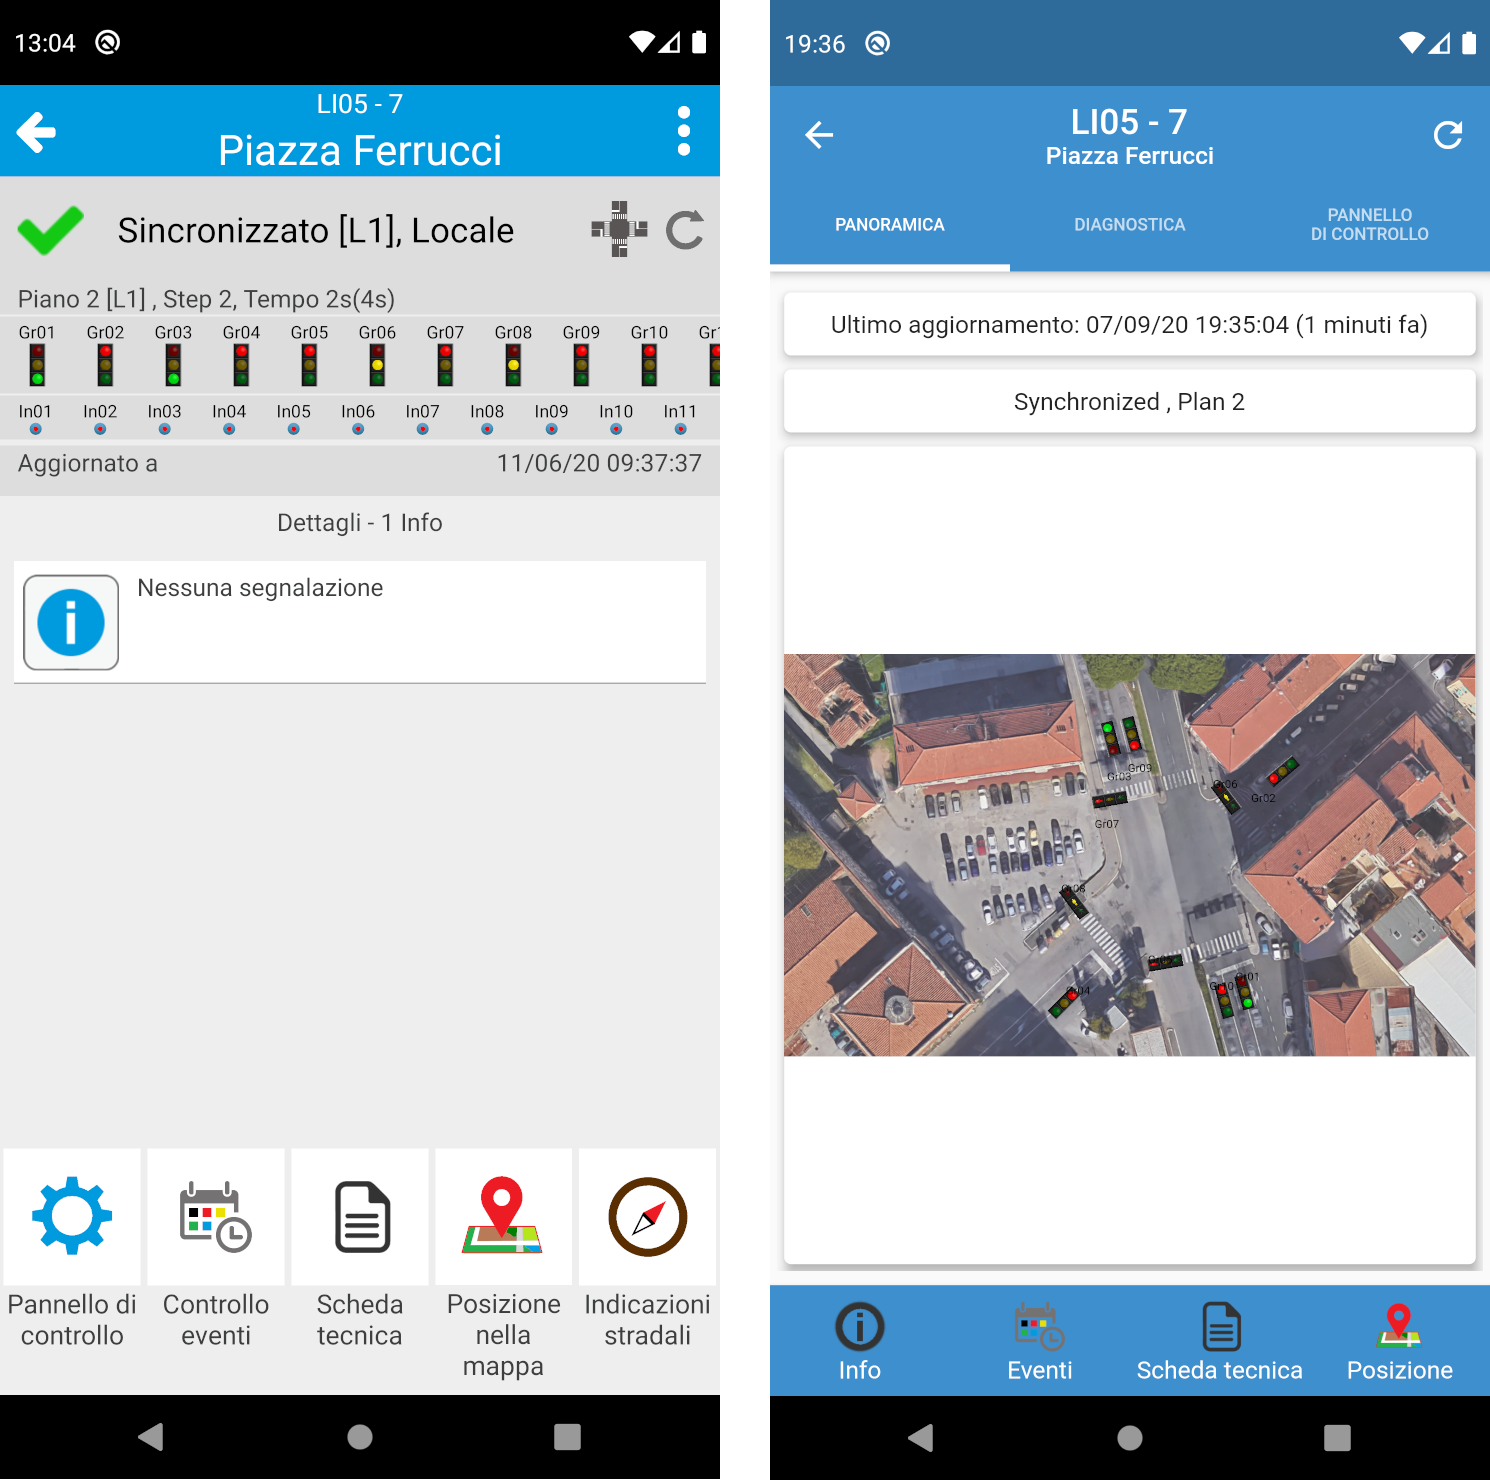
\includegraphics[width=1.0\columnwidth]{capitolo-6/confronto-app-vecchia-nuova/DeviceOverviewView} 
  \caption{Confronto fra schermate delle app: Panoramica sull'impianto}
\end{figure}